\appendix 
\chapter{Apéndice: teoría}


En este apéndice, establecemos las
definiciones y resultados
del álgebra y
de la teoría de espacios de Hilbert
estríctamente
necesarios para el desarrollo del trabajo.
A pesar de que los teoremas aquí expuestos son
clásicos, preferimos no limitarnos a simplemente citarlos
ya que queremos puntos de vista de estos tal vez
un poco distintos a los usuales, pero útiles para nosotros.

A menos que se
diga explícitamente lo contrario,
las elecciones del
orden en la exposición del material, 
al igual que las demostraciones
aquí contenidas, son personales. 



\section{Polinomios y teorema fundamental del álgebra}

En general, si $R$ es un anillo, se define a partir de 
él un nuevo anillo denominado el \textbf{anillo de polinomios
con coeficientes en $R$}; 
no vamos a ahondar en la construcción
algebráica de este (basada en sucesiones en $R$ de soporte
finito, c.f. \cite{jacobson} p.119), pero suponemos
que el lector está ya familiarizado con el anillo
$R[t]$, donde las operaciones de suma y multiplicación
se definen de la manera usual, así como con la noción
de evaluar un polinomio $f(t) \in R[t]$ en un elemento
$r \in R$ del anillo.


\begin{defi}
\label{def: coef principal y grado de un polinomio}
Sean $K$ un anillo, $f(t)= \suma{k=0}{n}{a_{k}t^{k}} \in K[t]$
con $a_{n}$ un elemento no cero del anillo $K$.
\begin{itemize}
\item Al elemento $a_{n} \in K$ se le llama el \textbf{coeficiente
principal} del polinomio $f$, y
\item a $n \in \overline{\IN}$ se le llama el \textbf{grado de $f$}
y se le denota por $\partial(f)$.
\end{itemize}
A todo elemento $r \in K$ tal que $f(r)=0$ se le llamará 
una \textbf{raíz de $f$}. 
\end{defi}


\begin{nota}
En \ref{def: coef principal y grado de un polinomio} se definió
el coeficiente principal y grado de todo polinomio no cero; 
por lo general, los algebristas prefieren definir el grado del 
polinomio cero como $-\infty$
(c.f. \cite{jacobson}, p.128) 
o dejarlo indefinido (c.f. \cite{rotman}, p.126).
Nosotros preferimos definir el grado del polinomio cero como
cero (que es el grado de todo polinomio constante). Esto lo hacemos
simplemente para no tener que distinguir al polinomio
cero como un caso especial, pues eso simplifica las formulaciones
de los resultados que necesitamos.
\end{nota}


\begin{prop}
\label{prop: grado producto polin}
(c.f. \cite{rotman}, p.127)
Si $K$ es un dominio entero, entonces, para cualesquiera
polinomios $f(t), g(t) \in K[t]$ no cero se tiene que
el producto $f(t) \cdot g(t)$ de estos dos polinomios no
es el polinomio cero y que
\[
\partial(f \cdot g) = \partial(f) \cdot \partial(g).
\]
\end{prop}

A nosotros nos interesará tomar siempre al anillo
de coeficientes $K$ como el campo $\IR$ o el campo $\IC$.

Es una consecuencia inmediata del algoritmo de la división
(c.f. \cite{rotman} p. 131) el que, si $K$ es un campo
y $f(t) \in K[t]$ es un polinomio de grado $n>0$, 
entonces $f$ tiene a lo más $n$ raíces (el argumento es
relacionar raíces de un polinomio con divisores lineales
de este y argumentar que, por 
\ref{prop: grado producto polin}, 
si el grado de $f$
es $n$ entonces $f$ no puede factorizarse como el producto
de más de $n$ factores lineales, luego, no puede tener más de 
$n$ raíces).

Se tiene pues una cota superior para la cantidad
de raíces de un polinomio no cero basada en 
su grado, sin embargo, esta cota bien puede no
alcanzarse. De hecho, como muestra el siguiente ejemplo,
puede ser que un polinomio no constante con coeficientes en un campo
no tenga ninguna raíz.

\begin{ejemplo}
Considere al anillo $\IZ_{5}$ de enteros módulo $5$. Como
$5$ es un número primo, $\IZ_{5}$ es un campo (c.f. proposición
3.12 de \cite{rotman}).
Sea $f(t)=t^{2}-2 \in \IZ_{5}[t]$; evaluar a este polinomio
en cada uno de los cinco elementos de $\IZ_{5}$
nunca da lugar al cero del campo, luego, $f$ es un polinomio
de grado dos con coeficientes en $\IZ_{5}$ sin raíces
(en $\IZ_{5}$).
\final
\end{ejemplo}

\begin{ejemplo}
El ejemplo canónico de polinomio con coeficientes reales
sin raíces (reales) es $p(t)=t^{2}+1 \in \IR[t]$. 
No puede tener raíces por
ser el cuadrado de todo número real no negativo. 
\final 
\end{ejemplo}



\begin{teo}
\label{teo: fundamental del algebra}
\textbf{(Teorema fundamental del álgebra, 
versión dada por \cite{kurosch}, p.149)}:
Todo polinomio
$f(t) \in \IC[t]$ de coeficientes complejos
y grado al menos uno
tiene al menos una raíz compleja.
\end{teo}

Como se hace notar en la referencia, es difícil exagerar
la importancia que tiene este teorema no sólo en el álgebra, 
sino en la matemática en general; se resalta también el hecho
de que, hasta el momento, todas las pruebas de este teorema
hacen uso no sólo de la estructura algebráica del dominio entero
$\IC[t]$, sino de propiedades
de otra índole (por ejemplo
topológicas) de
$\IC$ visto como un $\IC-$espacio vectorial
(obtenidas, por ejemplo, al definir en $\IC$ una norma, c.f.
\eqref{eq: producto punto Cn}).
Hay, sin embargo, construcciones puramente algebraicas
del campo $\IC$ basadas en la idea de ``completar'' al campo
de los números reales (c.f. \cite{godement}, 
\textit{L'anneau $K[\sqrt{d}]$}, p.152).


De un simple argumento inductivo, usando el teorema 
\ref{teo: fundamental del algebra} se demuestra que 
el que 
todo polinomio no constante con coeficientes en $\IC$
tenga al menos una raíz compleja \textbf{equivale} a que
tenga tantas raíces como su grado.

\begin{teo}
\label{teo: alt del fundamental del algebra}
Todo polinomio $f(t) \in \IC[t]$ 
de grado $n>0$
tiene exactamente $n$ raíces complejas
(contando multiplicidades).
\end{teo}
\noindent
\textbf{Demostración.}
Procedemos por inducción sobre $n$, el grado del polinomio.
Sea $f$ un polinomio con coeficientes
complejos y de grado $n=1$. Según el teorema 
\ref{teo: fundamental del algebra}, $f$ tiene al menos
una raíz $r_{1} \in \IC$, luego,
el polinomio lineal $x-r_{1}$
divide a $f$. Ahora bien, si $f$ tuviese una segunda
raíz $r_{2}$, el polinomio 
de grado dos $(x-r_{1})(x-r_{2})$
dividiría a $f$, pero esto contradice el que 
todos los divisores de un polinomio $f$ con coeficientes
en un campo tengan grado menor o igual al de $f$
(c.f. proposición \ref{prop: grado producto polin}). 
Con esto comprobamos la validez del teorema para $n=1$.

Supongamos ahora el teorema cierto para 
todo polinomio de grado
$n \geq 1$.
Sea $f \in \IC[t]$ un polinomio de grado $n+1$; según 
\ref{teo: fundamental del algebra}, $f$ tiene al menos
una raíz $r_{1}$, luego,
\begin{equation}
\label{eq0: 11Dic}
f(x)= (x-r_{1}) g(x), 
\end{equation}
con $g(x)$ algún polinomio de coeficientes complejos y grado
$n$ (c.f. proposición \ref{prop: grado producto polin}). 
Por hipótesis de inducción, $g$ tiene exactamente
$n$ raíces complejas (contando multiplicidades); puesto que,
según la ecuación \eqref{eq0: 11Dic}, las raíces de $f$
son $r_{1}$ y las raíces de $g$ (pues, en un campo, el producto
de dos elementos del campo es cero sí y sólo si alguno de 
estos es cero), concluimos, como queríamos, que, salvo
multiplicidades, $f$ tiene $n+1$ raíces complejas.
\null\nobreak\hfill\ensuremath{\square} 
\vspace{0.2cm}

La siguiente consecuencia inmediata del teorema fundamental del
álgebra es 
una de las piezas angulares del trabajo desarrollado en esta tesis.

\begin{prop}
\label{prop: cita TFA}
Sea $f(t) \in \IR[t]$ un polinomio con coeficientes reales
con $\partial(f) = n$. Si $f$ tiene más de $n$ raíces reales, entonces
$f$ es el polinomio cero.
\end{prop}
\noindent
\textbf{Demostración.}
En efecto, si $f$ tuviese grado mayor a cero, entonces, 
según el teorema \ref{teo: alt del fundamental del algebra},
$f$ tendría a lo más $n$ raíces reales,
pero, por hipótesis, $f$ tiene más de $n$; así, $f$
debe tener grado cero, o sea, debe  ser un polinomio constante.
Puesto que el único polinomio constante con al menos una raíz
es el polinomio cero, concluimos que $f=0$.
\null\nobreak\hfill\ensuremath{\square} %final dem
\vspace{0.2cm}
\section{Definiciones básicas}


\TODO{Yo creo que aquí debes de poner la def. de espacio
vectorial con producto punto y de espacio de Hilbert. Checa
la def. de Erwin y de Kolmogorov. Di además que
consideras que el producto punto es positive definite.} \\



Una de las
grandes ventajas de considerar
bases ortogonales sobre bases cualesquiera para un espacio es que
contamos con una fórmula sencilla
para los coeficientes de la representación lineal de los
elementos del subespacio que generan. Además, información
sobre tales coeficientes \TODO{asdfljka}.
En general. si $S$ es una base cualquiera para
el espacio $V$, los coeficientes no dan información
geométrica sobre el vector \TODO{aquí pon tu ejemplo
con las potencias.} \\
 
\TODO{recuerda poner aqu'los ejemplos canónicos
de espacio HIlbertiano que después cites...}

\TODO{$F \in \{ \IR , \IC \}$}. 
 
\TODO{Di que, dada la def. de producto punto, es natural definir la otrogonalidad y la
norma. Da la definición de base ortonormal (siendo la palabra 'base' usada
en el sentido usual)} 
 
 
\TODO{Por aquí da la nción de subespacio ortogonal, y explica
cómo este suma directamente con el original para formar
a todo el espacio ambiente.} 
 
\begin{defi}
Si $S=\{ w_{1}, \ldots , w_{n} \}$ es una base
ortogonal de $V$ y $v \in V$ cualquiera, a los
números
\[
\frac{\langle v , w_{k} \rangle}{\langle  w_{k}, w_{k} \rangle},
\hspace{1cm} 1 \leq k \leq n
\]
les llamaremos los \textbf{coeficientes de Fourier}
de $v$ respecto a la BO S.
\end{defi}

Observe que si la BO de la definición anterior de hecho
es una BON, entonces los coeficientes de Fourier de un 
vector $v$ respecto a esta no son más que los productos
puntos de $v$ con sus elementos.

\begin{prop}
Los coeficientes de Fourier de un vector $v$
respecto a una BO S son los coeficientes
de la combinación lineal de elementos de $S$ igual a $v$.
\end{prop}
\noindent
\textbf{Demostración.}
En efecto, si $v=\suma{i=1}{n}{c_{i}w_{i}}$,
la bilinealidad del producto punto y la hipótesis 
de ortogonalidad nos llevan a concluir que, 
para todo $k$,
\begin{align*}
\langle  v , w_{k} \rangle &= \langle \suma{i=1}{n}{c_{i}w_{i}}  , w_{k} \rangle \\
& = c_{1} \langle w_{1}  , w_{1} \rangle.
\end{align*}
\QEDB
\vspace{0.2cm}




\begin{ej} \label{ej: espacios con producto punto Rn y ell}
(de espacios con producto punto, que serán usados después en nuestro trabajo)

\textbf{Dimensión finita: $\IR^{n}$}. \TODO{aquí
la def del producto punto.}

\textbf{Dimensión infinita: $\ell^{2}(\IZ)$}. 
\[
\ell^{2}(\IZ) = \{ x=(x_{k})_{k \in \IZ} \in \IR^{\IZ} :
\suma{k \in \IZ}{}{|x_{k}|^{2} < \infty }\}.
 \]
 
Tenemos que hacer algunos comentarios sobre la forma
en que hemos expresado al clásico espacio $\ell^{2}(\IZ)$:

\begin{itemize}
	\item[(I)] $\IZ$ es un conjunto numerable,
	es decir, es posible establecer una biyección
	\[
	\begin{split}
	f: \IN & \longrightarrow \IZ \\
	k & \mapsto z_{k}.
	\end{split}
	\]
	Gracias a una tal $f$ podemos hablar de las sumas
	parciales $\suma{k=1}{n}{|x_{z_{k}}|^{2}}$ de una
	función $x \in \IR^{\IZ}$ y considerar el límite cuando 
	$n \rightarrow \infty $, permitiéndonos hablar de
	la serie $\suma{k \in \IZ}{}{|x_{k}|^{2}}$ que,
	por ser de términos no negativos, o bien converge a un 
	número real $L$ o bien diverge a $\infty$ (i.e. las sumas
	parciales pueden hacerse arbitrariamente grandes).
	En caso de converger o diverger, lo hace absolutamente, 
	luego, no importa cuál sera la biyección 
	$f: \IN \longrightarrow \IZ$ usada para formar
	las sumas parciales, estas siempre convergen a $L$
	o divergen, respectivamente. \TODO{cita el teorema
	correspondiente de Spivak}
	
	\item[(II)] Por lo general, por ``sucesión'' se 
	entiende una función de $\IN$ en $\IR$; sin embargo, lo único 
	que nos importa a nosotros sobre las sucesiones 
	$x: \IN \longrightarrow \IR$ es que
	\begin{enumerate}
		\item tienen un dominio discreto y numerable, y que
		\item el conjunto de sucesiones cuadrado-sumables
		es un $\IR$ -espacio vectorial. 
	\end{enumerate}
	Si en cambio consideramos funciones $x$ de
	$\IZ$ en $\IR$, seguiremos hablando de funciones
	con dominio discreto y numerable, y el conjunto
	de aquellas para las que la serie 
	$\suma{k \in \IZ}{}{|x_{k}|^{2}} $ sea convergente
	es también un espacio vectorial. La ventaja de usar
	a $\IZ$ como dominio es que esto hace de las funciones
	$x$ unas buenas candidatas para representar señales,
	pues no tendremos que preocuparnos por el inicio de
	una señal (dificultad que sí se presenta si por dominio
	se toma al conjunto acotado inferiormente $\IN$).
\end{itemize}



Según la desigualdad de Cauchy-Schwarz, para cualesquiera
$x, y \in \IR^{\IZ}$
\[
\left\lvert
\suma{k \in \IZ}{}{x_{k}y_{k}}
\right\rvert \leq
\left( \suma{k \in \IZ}{}{|x_{k}|^{2}} \right)^{1/2}
\left( \suma{k \in \IZ}{}{|y_{k}|^{2}} \right)^{1/2};
\]

es esta desigualdad la que justifica la buena definición
de la función 
	\[
	\begin{split}
	< , >: \ell^{2}(\IZ) \times \ell^{2}(\IZ) & \longrightarrow \IR \\
	(x,y) & \mapsto \suma{k \in \IZ}{}{x_{k}y_{k}};
	\end{split}
	\]

\TODO{Tengo un problema aquí. La serie involucrada para el producto
punto no es de términos positivos, luego, no aplica el argumento de 
antes para justificar que  ``podemos usar cualquier
orden (biyección)''.}

\noindent no es difícil comprobar que $< , >$ es un producto
punto en el espacio $\ell^{2}(\IZ)$. La norma que
induce está dada por la relación
\[
||x|| = \left[ \suma{k \in \IZ}{}{|x_{k}|^{2}} \right]^{\frac{1}{2}},
\hspace{0.8cm} x \in \ell^{2}(\IZ).
\]

\noindent Se demuestra en [\TODO{Kolmogorov}] que, salvo isometrías,
el espacio con producto interior $(\ell^{2}(\IZ), <, >)$
es el único completo, separable e infinito dimensional. \\


\begin{defi}
Si $\delta_{jk}$ es la delta de Kronecker asociada
a los enteros $j$ y $k$, o sea, el número real definido como
\begin{align*}
\delta_{jk} = \begin{cases}
1 & \text{ si } j=k \\
0 & o.c., 
\end{cases}
\end{align*}
entonces por $\delta_{j}$ denotamos al elemento 
de $\ell^{2}(\IZ)$ definido como

\[
\delta_{j}=(\delta_{jk})_{k \in \IZ}, 
\hspace{0.5cm} j \in \IZ.
\]
\end{defi}

\end{ej}


\section{Hiperplanos de espacios con producto punto de dimensión finita}
\label{section: hiperplanos}
En general, si $V$ es cualquier $F-$espacio vectorial (con $F$
un campo cualquiera) y $W$ es un subespacio de $V$
cuya dimensión difere de la del espacio ambiente $V$
por uno, $W$ se denomina un ''hiperplano`` de $V$.

Como a nosotros sólo nos interesa el escenario
en el que $V$ es finito dimensional y 
en él se ha definido un producto punto, damos la
definición para este caso
particular y algunas de sus consecuencias a continuación.

\begin{defi}
Sea $V$ un $\IR-$espacio vectorial,
con $dim(V)=n < \infty$ y con un producto punto $\langle \cdot, \cdot \rangle$
definido en él \footnote{\TODO{Por lo tanto un espacio
de Hilbert, i.e. completo, verdad?}}. A todo subespacio
$W$ de $V$ con $dim(W)=n-1$ le llamaremos un
\textbf{hiperplano de $V$.}
\end{defi}



Si $W$ es un hiperplano de $V$, puesto que
V=$W + W^{\perp}$
(c.f. \cite{friedberg}, p.355, ejercicio 13),
$W^{\perp}$ tiene dimensión uno; fijando pues un
vector $u$ de $W^{\perp}$, tenemos que
$W^{\perp}=span\{ u\}$. En base a este 
podemos definir (gracias a la linealidad
del producto punto) al siguiente funcional:

\begin{center}
\aplica{h_{u}}
{V}
{\IR }
{x}{\langle x, u \rangle.}
\end{center}
Observe que
\begin{itemize}
\item $h_{u}(x)>0$ si y sólo si $x= a u$ para algún $a>0$,
\item $h_{u}(x)=0$ si y sólo si $x \in W$,
\item $h_{u}(x)<0$ si y sólo si $x= a u$ para algún $a<0$.
\end{itemize}
Así, en base al hiperplano $W$, via
el funcional $h_{u}$ podemos dividir
al espacio ambiente $V$ en tres subconjuntos ajenos
dos a dos, a saber, 
\begin{equation}
\label{eq1: 29Nov}
R_{I}= \{ x \in V: \hspace{0.1cm} h_{u}(x)> 0 \},
\hspace{0.3cm}
R_{II}=W, 
\hspace{0.3cm}
R_{III}= \{ x \in V: \hspace{0.1cm} h_{u}(x)<0 \},
\end{equation}
siendo el funcional $h_{u}$ el criterio usado para
determinar la pertenencia de un $x \in V$ a alguna de estas regiones.

Es fácil comprobar que,
si se escoge otro vector $\tilde{u} \in W^{\perp}$,
las regiones análogas a las
\eqref{eq1: 29Nov} obtenidas ahora con el funcional
$h_{\tilde{u}}$ coinciden con las dadas en \eqref{eq1: 29Nov}
(aunque,
obviamente, pueden diferir en el orden en que estas se escriban),
pues todos los elementos de $W^{\perp}$ son múltiplos
escalares uno del otro.
En este sentido decimos que \textbf{todo hiperplano
divide en tres regiones ajenas al espacio ambiente.}




\section{El teorema de la proyección ortogonal}

En general, si $V$ es un espacio métrico y W es un subconjunto
de este, puede definirse la distancia de un punto $x \in V$ a W como
el ínfimo del conjunto de distancias entre $x$ y puntos de $W$:

\[
d(x,W)=inf\{d(x,y): y \in W \}.
\]
\noindent 
Tal ínfimo existe por estar el conjunto descrito acotado inferiormente,
por ejemplo, por el cero. El siguiente teorema nos dice que,
en el contexto de espacios de Hilbert, si $W$ es un subespacio de $V$
que además es cerrado \sidenote{Cuidado aquí: hay dos nociones distintas de 
cerradura involucradas. Como el espacio métrico $V$ es un espacio vectorial
normado, con ``subespacio'' nos referimos a un subespacio vectorial de $V$,
no a un mero subconjunto de este; es decir, requerimos que $W$ sea cerrado bajo
las operaciones de espacio vectorial. Se pide además que $W$ (pensado
como subconjunto del espacio métrico $V$) 
sea cerrado en el sentido topológico
(c.f. \cite{munkres} p.93 ).}, 
tal ínfimo se alcanza, es decir, existe un punto
(además, único) $\hat{x}$ de $W$ que minimiza la distancia a $x$. \\

\begin{teo} 
\label{Teo:proyOrt}
(\textbf{de la proyección ortogonal}
~\cite{Nimark}):
Sean $V$ un espacio de Hilbert, $W$ un subespacio cerrado de $V$. 
Para todo $x \in V$ existe un único $\hat{x} \in W$ tal que
\[
||x- \hat{x}|| = inf_{y \in W}|| x-y ||;
\]
además, $\hat{x}$ es el único elemento de $W$
tal que $x-\hat{x} \in W^{\perp} $.
\end{teo}


En este trabajo, 
el espacio con producto punto
particular que nos concierne 
es $\IR^{n}$ con el producto punto usual
(definido como en \eqref{eq: producto punto Rn}); por ser
este un espacio finito-dimensional, 
cualquier subespacio de este es cerrado
(c.f. teorema 2.4-3 de \cite{Kreyszig}),
luego, el teorema de la proyección siempre aplica. \\

En general, si $W$ es un subespacio cerrado de
un espacio de Hilbert $V$, gracias a la unicidad
establecida en el teorema \ref{Teo:proyOrt},
podemos definir la función \textbf{proyección a $W$}
como sigue:

\begin{equation}
\label{eq3: 1Dic}
\aplica{\Pi_{W}}{V}{W}{x}{\hat{x}},
\end{equation}
donde $\hat{x}$ es el único vector del que se habla
en el teorema \ref{Teo:proyOrt}.


Puede pensarse a esta como la función que a cada elemento
$x$ del espacio le asocia ``su representante'' del espacio $W$
más cercano. Otra consecuencia de la unicidad establecida en el teorema
\ref{Teo:proyOrt} es la linealidad de la función
$\Pi_{W}$. 

\begin{cor}
\label{cor: x como suma de proyecciones}
Sean $V$ es un espacio de Hilbert, $W$ un subespacio cerrado de 
$V$ cuyo complemento ortogonal también es cerrado en $V$.
Entonces,
\begin{itemize}
\item Para todo $x \in V$, $x= \Pi_{W}(x)+ \Pi_{W^{\perp}}(x)$.
\item $\Pi_{W}: V \longrightarrow W$ es un operador autoadjunto.
\end{itemize}
\end{cor}
\noindent
\textbf{Demostración.}
Sea $x \in V$ cualquiera; según el teorema
de la proyección
\ref{Teo:proyOrt}, 
\begin{equation}
\label{eq3: 1En}
x - \Pi_{W}(x) \in W^{\perp};
\end{equation}
además,
\begin{equation}
\label{eq4: 1En}
x-(x-\Pi_{W}(x))= \Pi_{W}(x) \in W \subseteq (W^{\perp})^{\perp};
\end{equation}
puesto que, según el teorema de la proyección, 
$\Pi_{W^{\perp}}(x)$ se caracteriza por ser el 
único elemento de $W^{\perp}$ tal que 
$x-\Pi_{W^{\perp}}(x) \in (W^{\perp})^{\perp}$,
concluimos por \eqref{eq3: 1En} y \eqref{eq4: 1En}
la igualdad
\[
x-\Pi_{W}(x)= \Pi_{W^{\perp}}(x).
\]
Esto demuestra el primer punto del corolario. Para demostrar
el segundo, o sea, que para cualesquiera
$x, y \in V$ se tiene que
\[
\langle x, \Pi_{W}(y) \rangle = 
\langle \Pi_{W}(x), y \rangle,
\]
sólo observe que,
usando el primer punto ya demostrado, tenemos que
\begin{align*}
\langle x, \Pi_{W}(y) \rangle = & 
\langle \Pi_{W}(x) + \Pi_{W^{\perp}}(x), \Pi_{W}(y) \rangle  \\
= & \langle \Pi_{W}(x), \Pi_{W}(y) \rangle  + 
\langle \Pi_{W^{\perp}}(x), \Pi_{W}(y) \rangle  \\
= & \langle \Pi_{W}(x), \Pi_{W}(y) \rangle  ,
\end{align*}
donde la última igualdad se da porque $\Pi_{W}(y) \in W$ y 
$\Pi_{W^{\perp}}(x) \in W^{\perp}$ (luego,
son vectores mutuamente perpendiculares), y, análogamente,
\[
\langle \Pi_{W}(x), y \rangle  =  
\langle \Pi_{W}(x), \Pi_{W}(y)\rangle .
\]
\QEDB
\vspace{0.2cm}

\begin{nota}
De hecho, una vez establecida la continuidad
del producto punto más adelante en la
proposición \ref{prop: continuidad del producto punto}, podremos
quitar en la formulación del corolario 
\ref{cor: x como suma de proyecciones}
la hipótesis de que $W^{\perp}$ sea cerrado, pues esto
será consecuencia de que $W$ lo sea; si $(a_{n})_{n \in \IN}$
es una sucesión en $W^{\perp}$ convergente a algún $a \in V$,
entonces, para todo $w \in W$,
$\langle a, w \rangle = 
\langle \limite{n \rightarrow \infty}{a_{n}}, w \rangle
= \limite{n \rightarrow \infty}{\langle a_{n},w \rangle}=
\limite{n \rightarrow \infty}{0}=0$,
luego, $a \in W^{\perp}$.
\end{nota}


\section{La desigualdad de Gram-Schmidt y la continuidad del producto punto}
\noindent Demostremos 
una de las desigualdades
más importantes con las que se cuenta en un espacio
con producto punto.

\begin{teo}
(\textbf{Desigualdad de Cauchy-Schwarz}) \label{Teo:CauchySchwarz}
Sea $F \in \{ \IR, \IC \}$.
Sea $V$ un $F-$espacio vectorial con producto punto 
$ \langle \cdot  , \cdot  \rangle$.
\begin{equation}
\label{eq0: 12Feb}
\forall x , y \in V : \hspace{0.5cm}
|\langle x , y \rangle | \leq ||x|| \cdot ||y||,
\end{equation}
siendo $|| \cdot ||$
la norma inducida por el producto punto.
\end{teo}
\noindent
\textbf{Demostración.}
(basada en la demostración
ofrecida en ~\cite{Lang}, p. 292)
\begin{itemize}
\item Si alguno de los vectores $x$ o $y$ es cero,
la igualdad se da trivialmente (el vector cero tiene norma
cero y es ortogonal a cualquier vector). 

\item Si $x=a y$ para algún $a \in F$ no cero, también se 
da la igualdad:
\[
|\langle  x , y \rangle | =
|\langle  ay , y \rangle | = |a| \cdot  |\langle  y , y \rangle | =  
 |a| \cdot ||y||^{2}
=||ay|| \cdot ||y|| = ||x|| \cdot ||y||.
\]
\item Supongamos por último que no ocurre ninguno
de los casos de los puntos anteriores, o sea, que
$x$ y $y$ son linealmente independientes. \\
Si $c:=\frac{\langle x , y \rangle}{\langle y , y \rangle}$,
de la linealidad en la primera entrada
del producto punto se sigue fácilmente que
$x - cy$ es ortogonal a $y$, por lo tanto, a $cy$,
luego, 
por el teorema de pitágoras,
\begin{align*}
||x||^{2} & = ||x-cy||^{2} + ||cy||^{2} \\
& \geq ||cy||^{2}= |c|^{2} \cdot ||y||^{2} \\
& = \frac{\langle x , y \rangle ^{2}}{\langle y , y \rangle ^{2}} \cdot\langle y , y \rangle
= \frac{\langle x , y \rangle ^{2}}{|| y ||^{2}},
\end{align*}
luego, 
\[
\langle x, y \rangle ^{2}  \leq ||x||^{2} \cdot ||y||^{2}.
\]
Tomando raíces cuadradas en ambos lados de la
desigualdad llegamos a la desigualdad deseada. \QEDB
\end{itemize}
\vspace{0.2cm}


Esta desigualdad, que relaciona la norma de los
vectores con el valor
absoluto de su producto punto, permite
establecer la continuidad del producto punto. \\


\begin{prop} \label{prop: continuidad del producto punto}
La función $\langle  \cdot , \cdot \rangle :
V \times V \longrightarrow \IR $ es continua.
\end{prop}
\noindent
\textbf{Demostración.}
Demostrar la continuidad de 
$\langle  \cdot , \cdot \rangle$ significa 
probar la veracidad de la implicación
\[
(x_{n}, y_{n}) \rightarrow (x,y) \hspace{0.5cm}
\Rightarrow \hspace{0.5cm} \limite{n \rightarrow \infty}{
\langle  x_{n} , y_{n} \rangle} = \langle  x , y \rangle .
\]
Hagamos esto. Puesto que
\[
x_{n} \rightarrow x \hspace{0.4cm} \text{y}
\hspace{0.4cm} y_{n} \rightarrow y, 
\]

\noindent
los módulos de los vectores $x_{n}$ y $y_{n}$ 
están acotados, digamos por las constantes $K$ y $M$. \\
Por la bilinealidad del producto punto, para toda $n$
\[
\langle x_{n}-x , y_{n}-y \rangle =
\langle x_{n}, y_{n}\rangle -
\langle x_{n} , y \rangle -
\langle x , y_{n} \rangle +
\langle x , y \rangle ,
\]
\noindent
luego, por la desigualdad triangular y la de Cauchy-Schwarz
(\ref{Teo:CauchySchwarz}),
\begin{align*}
0 & \leq |\langle x_{n}, y_{n}\rangle - \langle x , y \rangle|
& \leq & |\langle x_{n}-x , y_{n}-y \rangle| +
|\langle x_{n} , y \rangle| + |\langle x , y_{n} \rangle| \\
&& \leq & ||x_{n}-x|| \cdot ||y_{n}-y|| + ||x_{n}||\cdot ||y_{n}||
+||x|| \cdot ||y_{n}|| \\
&& \leq & ||x_{n}-x|| \cdot ||y_{n}-y|| + K\cdot ||y_{n}||
+M \cdot ||x||; 
\end{align*}
Como $x_{n} \rightarrow x$ y $y_{n} \rightarrow y$,
el lado derecho de la desigualdad tiende a cero
conforme $n \rightarrow \infty$. Por el teorema de la compresión,
concluimos que
\[
\limite{n \rightarrow \infty}{|\langle x_{n}, y_{n}\rangle - \langle x , y \rangle|}=0,
\]
o sea, que 
$ \limite{n \rightarrow \infty}{
\langle  x_{n} , y_{n} \rangle} = \langle  x , y \rangle$.
\QEDB
\vspace{0.2cm}


\begin{comment} Esto es algo que hice que, ahora sé, es incorrecto. \\ 
Una vez introducidas las proyecciones ortogonales, podemos
establecer la equivalencia entre nuestra definición de base ortonormal
de un espacio con producto punto y la dada en \TODO{Kolmogorov [--]}
(que corresponde al segundo punto del siguiente teorema);
esto nos interesa porque, en el desarrollo del trabajo, muchas
veces usaremos el punto de vista dado por este último.

\begin{teo}
Sean $V$ un espacio con producto punto $< , >$, $B=\{ x_{\alpha} \}_{\alpha \in \Delta}$
un subconjunto ortonormal de $V$. 
\TODO{de hecho, nunca usas la ortonormalidad.}
Las siguientes
proposiciones son equivalentes:
\begin{enumerate}
\item $B$ es BON de $V$ (o sea, todo elemento de $V$ puede
expresarse de forma única como combinación lineal finita de elementos de $B$,
i.e. $span(B)=V$)
\item El subespacio cerrado de $V$ más pequeño que contiene a $B$
es él mismo, o sea, 
\[
 \overline{B}= V,
\]
es decir, $B$ es denso en $V$ (\TODO{definición
válida en cualquier espacio topológico. Introduce antes la definición
general y la caracterización en términos de sucesiones de la cerradura
de un subconjunto cualquiera válida
en espacios métricos.}). \footnote{\TODO{en este caso se
dice que el sistema $B$ es completo, verdad?}}
\item $ \overline{span}(B)=V$.
\end{enumerate}
\end{teo}
\begin{dem}
Demostremos las equivalencias
\[
1) \Longleftrightarrow 3) \hspace{0.3cm} \text{y} \hspace{0.3cm}
3) \Longleftrightarrow 2). 
\]

\TODO{ya no estoy segura entre la equivalencia de 1 con 3. Recuerda
que el profesor te dijo que, en el caso inifinito dimensional, importan
más los subconjuntos densos a las bases del espacio (que siempre existen).
De todas formas, como usas el nombre ``base'', deberías aclarar
esto en la teoría.}

\begin{itemize}
\item[ $1) \Rightarrow  3)$] Sea $v \in V$; como
$B$ es base de este espacio, $v \in span(B)$, luego, 
$v$ es trivialmente elemento de la cerradura de $span(B)$.

\item[$3) \Rightarrow  1)$] Supongamos, por el contrario, que
$span(B) \subsetneq V $; sea pues $v \in V - span(B)$.
\TODO{no sé si aquí hay un error en el argumento; ¿cómo
estoy segura de que tal proyección existe? recuerda que el teorema
de la proyección ortogonal habla en términos de subespacios
CERRADOS.}
Sea $v':= \Pi_{span(B)}(v)$; puesto que $v'$ es elemento de 
$span(B)$ y $v$ no, estos son vectores distintos entre sí, luego,
\[
\epsilon := ||v-v'|| >0.
\]
Ahora bien, para este $\epsilon$, 
como span(B) es denso en $V$, existe $v'' \in span(B)$ tal que
\[
|| v-v'' || < \frac{\epsilon}{2};
\]
esto contradice el que $v'$ sea el elemento de $span(B)$ más
cercano a $v$.

\item[ $3) \Rightarrow  2)$]
Si $W$ es un subespacio cerrado de $V$ que contiene a $B$,
entonces también contiene a su span, luego, contiene a su cerradura, o sea, 
\[
V= \overline{span}(B) \subseteq W,
\]
luego, $W=V$.

\item[ $2) \Rightarrow  3)$] Puesto que el que un conjunto esté
contenido en otro implica que la cerradura del primero esté contenida
en la cerradura del segundo, tenemos que
\[
V = \overline{B} \subseteq \overline{span}(B) 
\subseteq \overline{V} =V. 
\]
\end{itemize}
\QEDB
\end{dem}
\end{comment}








\section{El teorema de Gram-Schmidt}

\begin{teo} \label{Teo:Gram-Schmidt}
\TODO{Mejor empieza a enumerar desde el cero!}
(\textbf{de Gram-Schmidt}): Sean $V$ un espacio vectorial
con producto punto, $S=\{ v_{1}, \ldots ,v_{n} \}$ un
subconjunto linealmente independiente de $V$. 
Defínanse los vectores

\[
\begin{split}
w_{1}:= & v_{1}, \\
w_{k} := & v_{k} - \suma{j=1}{k-1}{
\frac{\langle v_{k} , w_{j} \rangle}{
\langle w_{j} , w_{j} \rangle}  w_{j}},
\hspace{0.2cm} k=2, \ldots ,n;
\end{split}
\]
\noindent
$S'=\{ w_{1}, \ldots , w_{n} \}$ es un subconjunto
ortogonal que genera el mismo espacio que $S$. \TODO{[Friedberg]}
\end{teo}


La esencia del teorema de Gram-Schmidt es el reemplazar una base
$S=\{ v_{1}, \ldots ,v_{n} \}$ de un subespacio 
$U := span(S)$ cualquiera de $V$ 
por una base ortogonal $S'$ para este. \\
Muchas veces nos interesa normalizar a la base $S'$
para así obtener una base ortonormal del espacio; llamaremos
a este el ``proceso de ortonormalización de Gram-Schmidt'',
y lo abreviaremos como ``G-S''. \TODO{AA} \\

La ventaja de la formulación del Teorema
de Gram-Schmidt dada en \ref{Teo:Gram-Schmidt}
es que esta
da explícitamente la forma de calcular a los
vectores $w_{k}$, pero,
para nuestros fines, una formulación que
involucre proyecciones ortogonales sobre espacios
será preferible, pues de este modo la geometría
que hay detrás del proceso puede
vislumbrase mejor. 


\begin{prop} \label{Prop:Gram-Schmidt2}
\textbf{(versión del teorema de Gram-Scmidt en términos de
proyecciones)}
(\TODO{cambia la notación. Usa $v$ y $\xi$}.)
Sean $V$ un espacio vectorial con producto punto,
\[
S=\{ v_{1}, \ldots , v_{n}\}
\] un subconjunto
linealmente independiente de $V$ y
\[
S'=\{ w_{1}, \ldots , w_{n}\}
\] el subconjunto
ortogonal que resulta de aplicar el proceso de
Gram-Schmidt \ref{Teo:Gram-Schmidt} a $S$. \\
Si 
\[
W_{k}=span(v_{1}, \ldots , v_{k}), 
\]
con $k \in \{ 2, \ldots n\}$, entonces
\begin{center}
\framebox{ $w_{k+1}=v_{k+1}- \Pi_{W_{k}}(v_{k+1})$.}
\end{center}
\end{prop}
\noindent
\textbf{Demostración.}
Según el teorema de Gram-Schmidt (\ref{Teo:Gram-Schmidt}),
\[
W_{k}=span(w_{1}, \ldots , w_{k}).
\]
Si mostramos que
\begin{itemize}
	\item el vector $v_{k+1}-w_{k+1}$ es elemento
	del espacio $W_{k}$, y que
	\item $w_{k+1}=v_{k+1}-(v_{k+1}-w_{k+1})$
	es elemento de $W_{k}^{\perp}$,
\end{itemize}
por la unicidad establecida en
el teorema de la proyección ortogonal \ref{Teo:proyOrt}
podremos concluir la igualdad deseada. \\
Lo primero es claro, pues, según las fórmulas
dadas en el teorema \ref{Teo:Gram-Schmidt},
\[
v_{k+1}-w_{k+1}= 
\suma{j=1}{k}{
\left( \frac{v_{k} \cdot w_{j}}{w_{j} \cdot w_{j}} \right) w_{j}} \in W_{k}.
\]
Lo segundo se sigue de observar que
$w_{k+1}$ es ortogonal a los vectores $w_{1}, \ldots , w_{k}$;
como estos conforman una base para $W_{k}$, concluimos
que $w_{k+1} \in W_{k}^{\perp}$.
\begin{figure}[ht]
    \centering
    \incfig{ConFab}
\end{figure}

\QEDB
\vspace{0.2cm}

\newpage
\section{Ángulo entre elementos de un espacio con producto punto}
\label{angulo entre elementos de un espacio con producto punto}

Es gracias a la desigualdad de Cauchy-Schwarz
que es posible introducir una de las nociones
más valiosas con las que se cuenta en un espacio
vectorial con producto punto, a saber, la de ángulo entre dos
vectores.

Si $v$ y $w$ son dos elementos no cero de $V$, entonces,
según el teorema \ref{Teo:CauchySchwarz},
\[
-1 \leq \frac{\langle v, w \rangle}{||v|| \cdot ||w||} \leq 1,
\]
luego, puesto que la función coseno es una biyección
del intervalo $[0, \pi]$ al intervalo $[-1,1]$,
tenemos que existe un único elemento 
$\theta \in [0, \pi]$ tal que

\[
cos(\theta)= \frac{\langle v, w \rangle}{||v|| \cdot ||w||};
\]
a tal número $\theta$ se le denomina el 
\textbf{ángulo formado por los vectores $v$ y $w$}.

\begin{marginfigure}
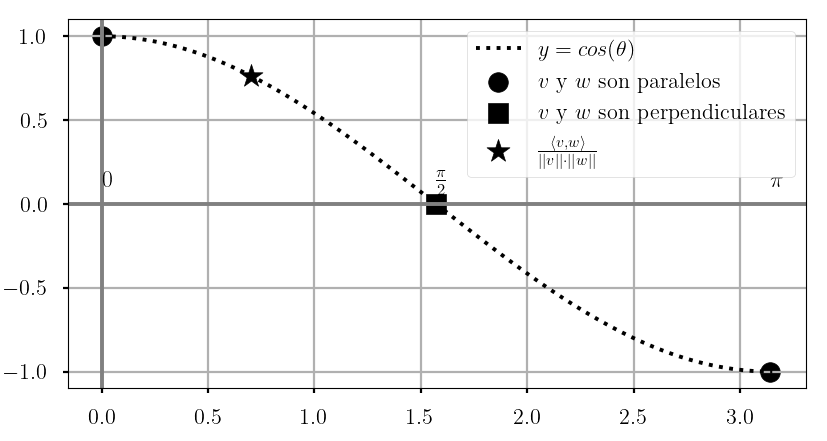
\includegraphics[scale=0.1]{coseno}
\end{marginfigure}

Si alguno de estos dos vectores fuese cero, definimos
el ángulo entre estos como cero. \TODO{Aquí deberías
de poner qué significan los casos extremos. Recuerda
la teoría de Spivak, cálculo en varias variables.}




\section{Definición de ángulo entre un punto y un subespacio en un espacio euclideo}

Ya vimos en \ref{angulo entre elementos de un espacio con producto punto}
cómo definir el ángulo entre dos elementos de un espacio
de Hilbert $V$.

Si además $W$ es un subespacio cerrado de $V$
(lo que, recuerde, siempre ocurre en caso de que
$V$ sea finito dimensional \TODO{ref.}), entonces también
es posible definir el ángulo entre un punto $x \in V$
del espacio y $W$.

\begin{defi} \label{def: angulo punto subespacio}
Sea $(V, \langle \cdot , \cdot \rangle)$ un espacio con 
producto punto. Sean $W \leq V$ un subespacio cerrado de $V$
y $x \in V$. Definimos el \textbf{ángulo entre $x$ y $W$}
como el ángulo que forma 
$x$ con su proyección a $W$, es decir,
\[
\measuredangle (x, W):= \measuredangle(x, \Pi_{W}(x)).
\]
\end{defi}

Una definición alternativa del ángulo entre un punto y un subespacio,
así como una caracterización sencilla del coseno de este,
se dan a continuación.

\begin{prop}
\label{prop: algunos hechos sobre el angulo entre un vector y un subespacio}
Si $V$, $W$ y $x$ son como en la definición 
\ref{def: angulo punto subespacio}, entonces

\begin{itemize}
\item \[
\measuredangle (x, W) = min \{ \measuredangle(x,w) \hspace{0.1cm} :
 \hspace{0.1cm} w \in W \},
\]
y 

\item $cos \left( \measuredangle (x, W) \right) = \frac{|| \Pi_{W}(x) ||}{||x||}$.
\end{itemize}


\end{prop}
\noindent
\textbf{Demostración.}
\begin{itemize}
\item  Sea $w$ un elemento cualquiera de $W$.
Puesto que el ángulo entre dos vectores es
preservado bajo multiplicación por escalares
(c.f. \TODO{debes poner en el apéndice este resultado, 
luego lo citas en el ejemplo}), sin pérdida de generalidad
podemos suponer que 
\begin{equation}
\label{eq1: 9Feb}
||w||= || \Pi_{W}(x)||.
\end{equation}

De la definición del vector $\Pi_{W}(x)$ se sigue que
\[
|| x -\Pi_{W}(x) ||^{2} \leq  || x - w||^{2};
\]
expresando ambos lados de la desigualdad como un producto
punto (c.f. \TODO{referencia}) y aplicando la
bilinealidad del producto punto, llegamos a que
\[
\langle x , x \rangle -2 \langle x, \Pi_{W}(x) \rangle +
\langle \Pi_{W}(x) , \Pi_{W}(x) \rangle \leq 
\langle x , x \rangle  -2 \langle x , w \rangle 
+ \langle w , w \rangle ;
\]
usando \eqref{eq1: 9Feb}, podemos simplificar esta
última desigualdad para llegar a 
\[
\langle x, w \rangle \leq \langle x, \Pi_{W}(x) \rangle,
\]
de donde se sigue, usando nuevamente \eqref{eq1: 9Feb},
que 
\[
cos \left( \measuredangle (x,w) \right) =
\frac{\langle x , w \rangle}{||x||\cdot ||w||} \leq
\frac{\langle x ,  \Pi_{W}(x)  \rangle}{||x||\cdot ||w||} =
cos \left( \measuredangle \left(x, \Pi_{W}(x) \right) \right);
\]
del que la función coseno sea decreciente en el intervalo
$[0, \pi]$ se concluye de esta última desigualdad que
$ \measuredangle \left(x, \Pi_{W}(x) \right) \leq 
\measuredangle (x,w)$.

\item Según el corolario 
\ref{cor: x como suma de proyecciones}, 
$x$ puede expresarse como la suma entre su proyección
a $W$ y su proyección a $W^{\perp}$, luego,
según la definición \ref{def: angulo punto subespacio}
y la linealidad del producto punto, concluimos que

\begin{align*}
cos \left( \measuredangle (x, W) \right) = &
cos \left( \measuredangle (x, \Pi_{W}(x)) \right)  \\
= & 
\frac{\langle x , \Pi_{W}(x) \rangle}{||x|| \cdot || \Pi_{W}(x)||}  \\
= & 
\frac{\langle \Pi_{W}(x)+\Pi_{W\perp}(x) , \Pi_{W}(x) \rangle}{||x|| \cdot || \Pi_{W}(x)||}\\
= & \frac{\langle \Pi_{W}(x) , \Pi_{W}(x) \rangle}{||x|| \cdot || \Pi_{W}(x)||}\\
= & \frac{|| \Pi_{W}(x) ||^{2}}{||x|| \cdot || \Pi_{W}(x)||}\\
= & \frac{|| \Pi_{W}(x) ||}{||x||}.
\end{align*}
\end{itemize}

\QEDB
\vspace{0.2cm}


\TODO{Deberías de exĺicar por qué $\measuredangle (x, W) \in [0, \frac{\pi}{2}]$
y no $\measuredangle (x, W) \in [0, \pi]$.}

\TODO{Pon ejemplos gráficos en dimensión 2 y 3.
Creo que en dimensión 2 el ángulo entre $x$ y un vector
de $W$ es siempre el mismo.}


\subsection{Cosine similarity}
\label{cosine similarity}

Sea $V$ un espacio euclideo. \TODO{Ve si siempre usas este
nombre. Creo que siempre lo cambias jaja.}
Sean $W \subseteq V$ un subespacio cerrado de $V$ y 
$x$ un elemento cualquiera de $V$. Hay dos formas ``naturales''
de intentar medir la cercanía de $x$ a $W$:
\begin{itemize}
\item[a)] \textbf{Usando la distancia euclidea
de $x$ a $W$}, es decir, tomando la norma del vector
$x - \Pi_{W}(x)$ (\TODO{referencia que diga que así se mide
la distncia. Tal vez Ana Irene lo tenga.}) como una medida
de qué tanto pertenece $x$ a $W$.
\item[b)] \textbf{Usando el ángulo que $x$ forma con $W$}: como ya
vimos en la sección \TODO{ref.}, el ángulo 
$\measuredangle (x, W) \in [0, \frac{\pi}{2}]$
entre $x$ y $W$
está definido como el ángulo entre $x$ y su proyección
$\Pi_{W}(x)$ a $W$, luego, 
	\begin{itemize}
		\item entre más cercano a cero sea $\measuredangle (x, W)$,
		$x$ se aleja más del plano $W$, pues es casi perpendicular 
		al elemento de $W$ más cercano a $x$, y
		
		\item entre más cercano a uno sea $\measuredangle (x, W)$,
		más se acerca $x$ a ser paralelo a su representante en $W$,
		luego, más se acerca $x$ a pertenecer a $W$.
	\end{itemize}
\end{itemize}

\begin{figure}[H]
	\sidecaption{
	Esquema de dos formas en las que uno puede intentar medir
	qué tan afín es una señal $x$.
	\label{fig: dos formas de medir distancia a plano}
	}
	\centering
	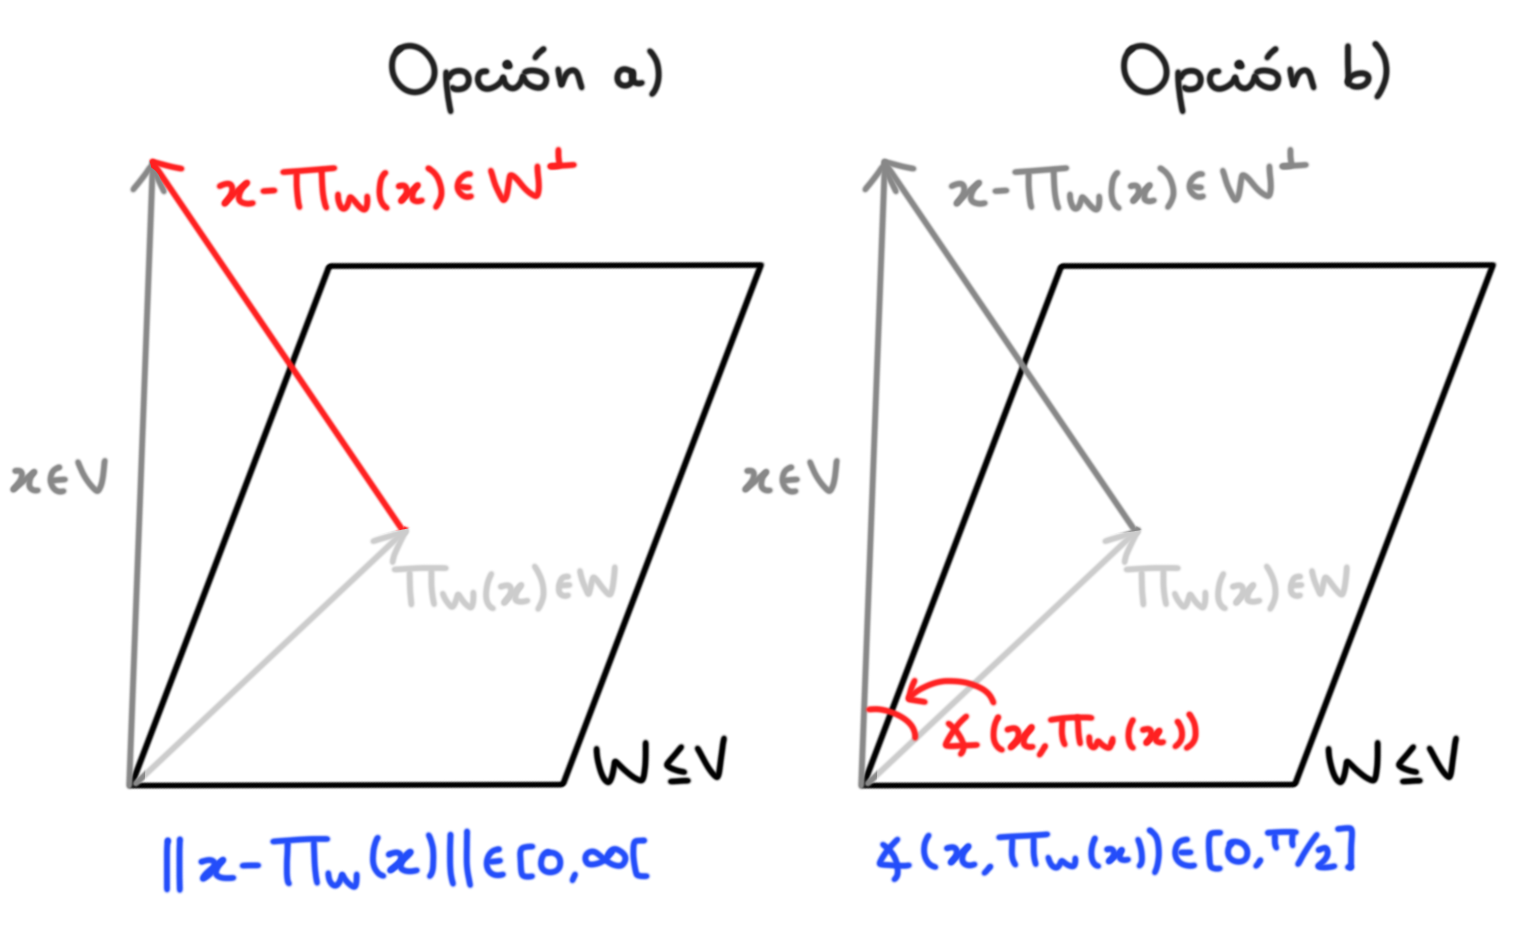
\includegraphics[scale= 1]{ 18Sept_1} 
\end{figure}	

El primer enfoque se basa en la definición de distancia de $x$
a $W$; el segundo, en el ángulo que $x$ forma con $W$. Este segundo
enfoque es conocido como ``\textbf{cosine similarity}'' en
inglés (c.f. \TODO{ref. wikipedia}). Una ventaja que será clave
para nosotros del segundo método sobre el primero se
expone en el siguiente resultado.


\begin{prop}
\label{prop: angulo se conserva bajo mult. esc.}
Sean $V$ un espacio euclideo, $W \subseteq V$ cerrado, $x \in V$,
$a \in \IR - \{ 0 \}$. Si $|a| \neq 1$, la distancia euclídea 
de $a \cdot x$ a $W$ es distinta
a la de $x$ a $W$, mientras que el ángulo que forman $a \cdot x$ y $x$
con $W$ es el mismo.
\end{prop}
\noindent
\textbf{Demostración.}
En efecto, 

\[
|| a \cdot x - \Pi_{W}(a \cdot x) || = |a| \cdot || x - \Pi_{W}(x) ||, 
\]
y

\begin{align*}
\measuredangle (a \cdot x, W_{n,1}):=& \measuredangle(a \cdot x, \Pi_{W_{n,1}}(a \cdot x)) \\
= & \frac{\langle a \cdot x , \Pi_{W_{n,1}}(a \cdot x) \rangle}{|| a \cdot x || \cdot 
|| \Pi_{W_{n,1}}(a \cdot x)  ||} \\
= & \frac{a^{2}  \langle   x , \Pi_{W_{n,1}}(x) \rangle}{a^{2} ||  x || \cdot 
|| \Pi_{W_{n,1}}( x)  ||}  \\
= & \measuredangle (x, W_{n,1}).
\end{align*}


\QEDB
\vspace{0.2cm}

Así el criterio $b)$ no se ve afectado por multiplicación escalar,
mientras que el $a)$ sí.
 

\subsection{Caso particular en el que el subespacio en cuestión es un plano}
\label{ap: Caso particular en el que el subespacio en cuestión es un plano}

Para terminar este apartado, vamos a
agregar unos resultados que serán usados en la teoría
\TODO{mejora descripción.}


La situación es la siguiente: $V$ es un $\IR-$espacio
de Hilbert, $u$ y $v$ son elementos de $V$,
unitarios y linealmente
independientes entre sí. El espacio que ellos generan
es pues un plano, digamos,


\[
P= span \{ u, v \}
\]

Dado $x \in V$ unitario, nos gustaría dar una medida
de la cercanía de $x$ con el espacio $P$; si tomamos
al coseno del ángulo como una tal medida, según la proposición
\ref{prop: algunos hechos sobre el angulo entre un vector y un subespacio},

\begin{equation}
\label{eq0: 19Marzo}
cos \left( \measuredangle (x, P) \right) = || \Pi_{P}(x) ||;
\end{equation}
para lograr expresar el lado derecho de la igualdad en términos
sólo de $u$, $v$ y $x$ (que son los elementos básicos de
nuestra discusión), conviene primero considerar una base
ortonormal del espacio $P$.


\begin{obs}
Si $u, v \in V$ son unitarios y linealmente independientes, y $P$
es el plano que generan, entonces
$\{ u, z \}$, donde

\begin{equation}
\label{eq2: 19Marzo}
z:= \frac{v- \langle u, v \rangle u}{||v- \langle u, v \rangle u||}
\end{equation}
es una BON de $P$
\end{obs}
\noindent
\textbf{Demostración.}
Basta aplicar el teorema de Gram-Schmidt 
\ref{Teo:Gram-Schmidt}.
\QEDB
\vspace{0.2cm}

Teniendo una BON de $P$ se obtiene, via la prop.
y la expresión \eqref{eq0: 19Marzo},
\TODO{ref; debes de poner la discusión de BON mucho antes!!}
se obtiene una expresión de la proyección de $x$ al plano $P$ en función
de $x$, $u$ y $z$;

\begin{equation}
\label{eq1: 19Marzo}
\Pi_{P}(x)= \langle x, u \rangle u + \langle x, z \rangle z;
\end{equation}

puesto que, según la definición \eqref{eq2: 19Marzo} de 
$z$ este vector es función de $u$ y $v$, fácilmente se
deriva una expresión de $\Pi_{P}(x)$ (y, por lo tanto, una
medida de la cercanía de $x$ al plano $P$) en función sólo
de $x$, $u$ y $v$.

	\begin{prop}
	\label{prop: formulas 20Marzo}
	si $x, u, v \in V$ y $P \subseteq V$ son como en la discusión anterior
	(\TODO{pon aquí las hipótesis!}),
	entonces 

		\begin{equation}
		\label{eq3: 19Marzo}
		\Pi_{P}(x)= \frac{\langle x, u \rangle -\langle u, v \rangle \langle x, v \rangle }{1-\langle u, v \rangle^{2}} u + \frac{\langle x, v \rangle -\langle u, v \rangle \langle x, u \rangle }{1-\langle u, v \rangle^{2}} v
		\end{equation}
	y 
		\begin{equation}
		\label{eq3: 19Marzo}
		  || \Pi_{P}(x) ||^{2}=
		  \frac{1}{1- \langle u, v \rangle^{2}} \left(  
	       \langle x, u \rangle^{2} +  \langle x, v \rangle^{2}	
	       -2  \langle x, u \rangle^{2} \langle x, v \rangle^{2} \langle u, v \rangle^{2}	  
		  \right).
		\end{equation}
 
	\end{prop}


\section{Bases ortonormales de espacios de Hilbert}
\label{Bases ortonormales de espacios de Hilbert}

En general, dado un $F-$espacio vectorial $V$,
si uno acepta el axioma de elección, siempre cuenta con 
bases para este espacio,
es decir, de subconjuntos de $V$ que son tanto linealmente
independientes (término abreviado como ``l.i.'') como generadores
de todo el espacio; la importancia de 
estas es obvia pues, por definición, una base permite representar
de forma única a un elemento $v \in V$ por medio
de una colección de escalares. 


Puede demostrarse
que, dado $A \subseteq V$, el que $A$ sea base de $V$
equivale a que $A$ sea un maximal linealmente
independiente (c.f. sección 1.7 de \cite{friedberg}), es decir,
que todo subconjunto  linealmente
independiente de $V$ que contenga
a $A$ de hecho coincide con $A$.


El tener además en $V$ definido un producto punto
dota de estructura extra al espacio, en particular, 
como dijimos ya,
nos provee de una noción de longitud (\TODO{ref}) y también 
de ortogonalidad (\TODO{ref}), luego, en este 
contexto podemos también hablar de subconjuntos $B$
ortonormales maximales. Puesto que la ortogonalidad implica
trivialmente la independencia lineal, es natural plantearse
la siguiente pregunta: en un $F-$espacio vectorial $V$
con producto punto
cualquiera, ¿es cierto que todo ortonormal maximal es también
maximal l.i., o sea, una base
del espacio? 

Antes de proceder, 
conviene dejar por escrito estos dos conceptos.

\begin{defi} \label{defi: BON y base de Hamel}
Sea $V$ un espacio vectorial con producto punto.
Si $A$ es un subconjunto de $V$ que es 
maximal con respecto a la propiedad de
\begin{itemize}
\item ser linealmente independiente, entonces lo llamaremos
\textbf{base de Hamel} de $V$
\item ser ortonormal, entonces lo llamaremos
\textbf{base ortonormal} de $V$ (y abreviamos este
nombre como \textbf{BON}).
\end{itemize}
\end{defi}


Como se establece 
fácilmente en la siguiente proposición,
\textit{en el caso finito dimensional}, la respuesta a la pregunta
planteada es positiva.

\begin{prop}
\textbf{(en espacios de Hilbert de dimensión finita, toda BON es
base de Hamel)}
\label{prop: en dimension finita toda BON es base de Hamel}
Sea $V$ un espacio finito dimensional
con producto punto. Si $A$
es un subconjunto ortonormal maximal de $V$, entonces
también es maximal l.i. (o sea, base de $V$)
\end{prop}
\noindent
\textbf{Demostración.}
Supongamos que $A \subseteq V$ es maximal 
respecto a la propiedad de ser ortonormal pero
no a la de ser l.i., es decir, que existe
un subconjunto $A'$ l.i. que contiene a $A$ propiamente.
Digamos que $A' = A \cup B$.
Podemos ortonormalizar a este con el proceso de Gram-Schmidt
para obtener un subconjunto ortonormal $A´´$ de
$V$ que genera 
el mismo espacio que genera $A'$;
por las fórmulas del teorema \ref{Teo:Gram-Schmidt}
y el hecho de que los elementos de $A$ sean ortogonales
entre sí es claro que los primeros $|A|$ elementos
son los elementos de $A$ (``intactos''); así $A''$
es un subconjunto ortonormal de $V$ que contiene propiamente
a $A$ (contradicción).
\QEDB
\vspace{0.2cm}


Como se comenta en \cite{mse1},
en el caso en el que el espacio de Hilbert $V$
no sea infinito-dimensional, \textbf{una base 
Hamel de este espacio no puede ser una
base ortonormal del espacio.}

Así, en general los sistemas de representación
descritos en la definición 
\ref{defi: BON y base de Hamel} no son equivalentes.
A pesar de que
\begin{itemize}
	\item todo espacio de Hilbert tiene bases de Hamel, aunque
	no necesariamente bases ortonormales (c.f. 
	\cite{mse2}), y que
	
	\item si $\cali{B}$ es una base Hamel uno \textit{siempre}
	puede representar cualquier vector $x$ del espacio como combinación
	lineal \textit{finita} de elementos de $\cali{B}$, mientras que,
	si $\cali{B}$ es una BON, se tienen no igualdades entre 
	$x$ y combinaciones lineales de elementos de $\cali{B}$, sino aproximaciones
	del primero a partir de los segundos (c.f. inciso d)
	del teorema \ref{thm: Coway, 4.13}),
\end{itemize}

\noindent
como mostraremos más adelante, en el contexto de
espacios de Hilbert, conviene mucho más trabajar con BONs
(cuando existen para el espacio particular)
que con bases de Hamel. 


Es por eso que en la mayoría
de los libros de análisis funcional, el nombre ``base''
suele ser sinónimo de 
``base ortonormal''
(pudiendo llegar a confundir
a un lector primerizo, y llevarlo a pensar en
bases de Hamel). Puesto que
nosotros no queremos dar lugar a confusiones de este estilo,
nos abstenemos de usar el nombre ``base'', y en su lugar ocupamos
los nombres introducidos en la definición \ref{defi: BON y base de Hamel}.


\TODO{Espacio de Hilbert = espacio con producto punto completo, verdad?
Cambia además H por V. Recuerda que debes introducir el concepto
de ``nets'' de Munkres.}
\begin{teo} \label{thm: Coway, 4.13}
\textbf{(Teorema 4.13 de \cite{conway} )}
Sea $\cali{E}$ un subconjunto ortonormal del espacio
de hilbert $\cali{H}$.
Las siguiente proposiciones son equivalentes entre sí:
\begin{itemize}
\item[a)] $\cali{E}$ es una BON de $\cali{H}$.
\item[b)] Si $h \in \cali{H}$ es ortogonal a todo elemento de 
$\cali{E}$ entonces es cero.
\item[c)] $\overline{span}(E)= \cali{H} $.
\item[d)] Para todo $h \in \cali{H}$ se cumple que
\[
h = \suma{}{}{\{ <h,e> e | e \in \cali{E} \}}
\]
\item[e)] Para cualesquiera $g, h \in \cali{H}$,
\[
<g,h>= \suma{}{}{\{ <g,e> <e,h> | e \in \cali{E} \}}
\]
\item[f)](\textbf{Identidad de Parseval})
Para todo $h \in \cali{H}$ se cumple que
\[
||h||^{2}= \suma{}{}{\{ <h,e>^{2} | e \in \cali{E} \}}.
\]
\end{itemize}
\end{teo}

\sidenote{
El inciso $c)$ del teorema 
\ref{thm: Coway, 4.13}
corresponde a la definición
de BON dada en \cite{kolmogorov}; así, una BON
es también un subconjunto ortonormal tal que el menor
subespacio cerrado de $\cali{H}$ que contiene a $E$ es 
todo $\cali{H}$. Compare este inciso con el hecho de que
$E$ es una base de Hamel de $V$ si y sólo si $E$ es
linealmente independiente y $span(E) = V$.}
\noindent
\textbf{Demostración.}
\begin{itemize}
\item[$a) \Rightarrow b)$] Suponer la existencia de un 
$h$ no cero ortogonal a todo elemento de $\cali{E}$
nos permite considerar al subconjunto ortonormal
\[
\cali{E} \cup \{ \frac{h}{||h||} \}
\]
de $\cali{H}$
que contiene propiamente a $\cali{E}$,
contradiciendo así la maximalidad de $\cali{E}$.

\item[$b) \Rightarrow c)$] Sea el subespacio
$W := \overline{span}(E)$ de $\cali{H}$. Por ser
$W$ un subespacio cerrado de $\cali{H}$, podemos proyectar
sobre él. Para mostrar que tenemos la igualdad entre
estos dos espacios, tomemos un $h \in \cali{H}$ cualquiera.
Según el teorema de la proyección ortogonal 
\ref{Teo:proyOrt}, $(h-\Pi_{W}(h))$
es ortogonal a todo elemento de $W$, 
a todo elemento de $E$;
por hipótesis, esto implica que $h-\Pi_{W}(h)$ sea el vector cero.
Así,
\[
h = \Pi_{W}(h) \in W.
\]

\item[$c) \Rightarrow b)$] Sea $h \in \cali{H}$
ortogonal a todo elemento de $\cali{E}$; mostremos que
$h$ es cero. Como $h \in \overline{span}(E)$ (hipótesis),
existe $(b_{n})_{n \in \IN}$ una sucesión de
$span(E)$ tal que
$\lim_{n \rightarrow \infty}b_{n}=h$.
Usando el que para toda $n$ el producto punto $<b_{n}, h>$
sea cero y la continuidad
establecida en la proposición \ref{prop: continuidad del producto punto},
llegamos a que
\[
<h,h>= <h, \lim_{n \rightarrow \infty}b_{n}>= 
\lim_{n \rightarrow \infty}b_{n}<h, b_{n}>= 
\lim_{n \rightarrow \infty} 0 = 0,
\]
de donde concluimos que $h=0$.


\item[$b) \Rightarrow d)$] Según el \TODO{Lema 4.12},
la red $\suma{}{}{\{ <h,e>e | e \in \cali{E} \}}$
en efecto converge a un vector; resta ver que tal 
vector es $h$
o, equivalentemente, que
\begin{equation} \label{eq 0: 8Agosto}
h- \suma{}{}{\{ <h,e>e | e \in \cali{E} \}}
\end{equation}
es el vector cero; según nuestra hipótesis, podremos
concluir esto si demostramos que para todo $e \in \cali{E}$
ocurre
\[
<e, \suma{}{}{\{ <h,e>e | e \in \cali{E} -h \}} > =0.
\]
Haremos esto mostrando que la norma de 
\eqref{eq 0: 8Agosto} es cero \\
Sea $\epsilon >0$.
Por definición de convergencia de redes, sabemos que
existe $F \subseteq \cali{E}$ finito con $e \in F$
tal que
\begin{equation} \label{eq 1: 8Agosto}
|L_{F}| < \epsilon,
\end{equation}
donde $L_{F}:= \suma{f \in F}{}{<h,f>f} - 
\suma{}{}{\{ <h,e>e| e \in \cali{E} \}}$. \\

Por la bilinealidad del producto punto y por
ser $e$ ortogonal a todo elemento de $\cali{E}-\{ e \}$
tenemos que
\begin{equation} \label{eq 2: 8Agosto}
<\suma{f \in F}{}{<h,f>f}, e> = \suma{f \in F}{}{<h,f><f,e>}
= <h,e> <e,e>=<h,e>.
\end{equation}

Así,
\begin{align*}
0 \leq |<e, \suma{}{}{\{ <h,e>e | e \in \cali{E} \}} -h > | = &
| <e, \suma{}{}{\{ <h,e>e | e \in \cali{E} \}} > - <e,h>| = \\
=  | <e, \suma{}{}{\{ <h,e>e | e \in \cali{E} \}} - \suma{f \in F}{}{<h,f>f}
+ & \suma{f \in F}{}{<h,f>f} > - <h,e> | \\
= & | <e,  \suma{f \in F}{}{<h,f>f}> + <e, L_{F}> - <h,e>  | \\
(\text{por \eqref{eq 2: 8Agosto} }) = & |<e, L_{F}>| \\
(\text{Cauchy-Schwarz})&   \leq |e| |L_{F}| = |L_{F} | \\
(\text{por \eqref{eq 1: 8Agosto}})& < \epsilon.  
\end{align*}


Demostramos entonces que
\[
(\forall \epsilon > 0): \hspace{0.5cm} 
0 \leq |<e, \suma{}{}{\{ <h,e>e | e \in \cali{E} \}} -h > |< \epsilon;
\]
de esto conlcuimos que $|<e, \suma{}{}{\{ <h,e>e | e \in \cali{E} \}} -h > |$
es cero.

\item[$d) \Rightarrow e)$] Según nuestra hipótesis,
\[
h= \suma{}{}{\{ <h,e>e | e \in \cali{E} \} }, \hspace{0.5cm}
g= \suma{}{}{\{ <g,e>e | e \in \cali{E} \} }.
\]

Para $F \subseteq \cali{E}$ finito, sean
\[
H_{F}:= \suma{e \in F}{}{<h, e>e-h},
\hspace{0.5cm}
G_{F}:= \suma{e \in F}{}{<g, e>e-g}.
\]

Por la ortonormalidad supuesta en el conjunto $\cali{E}$,
\begin{equation}
\label{eq 3: 8Agosto}
<\suma{e \in F}{}{<h, e>e}, \suma{e \in F}{}{<g, e>e} >
= \suma{e \in F}{}{<h,e><g,e>};
\end{equation}
así,
\begin{align*}
|\suma{e \in F}{}{<h,e><g,e>} - <h,g>| \underbrace{=}_{\text{por 
\eqref{eq 3: 8Agosto}}} & |<\suma{e \in F}{}{<h, e>e}, \suma{e \in F}{}{<g, e>e} >
- <h,g>| \\
= & |<H_{F}+h, G_{F}+g > - <h,g>| \\
= & |<H_{F}, G_{F}> -<H_{F}, g> + <h,G_{h}>| \\
(\text{desigualdad triangular}) \leq & |<H_{F}, G_{F}> | + |<H_{F}, g>|
+ |<h,G_{H}>| \\
(\text{Cauchy-Schwarz}) \leq & ||H_{F}|| \cdot ||G_{F}|| +
||H_{F}|| \cdot ||g|| + ||h|| \cdot ||G_{H}||;
\end{align*}
puesto que $||g||$ y $||h||$ son constantes
y $||H_{F}||$ y $||G_{F}||$ pueden hacerse tan pequeñas como
se quiera (escogiendo apropiadamente al conjunto finito $F$),
concluimos que la red 
$\suma{}{}{\ <h,e> <g,e> | e \in \cali{E}\}}$
converge a $<h,g>$.

\item[$e) \Rightarrow f)$] Para $h \in \cali{H}$,
\[
||h||^{2}=<h,h> = \suma{}{}{\{ <h,e>^{2}| e \in \cali{E} \}}.
\]

\item[$e) \Rightarrow f)$]
Supongamos que $\cali{E}$ puede extenderse aún más
para ser ortonormal, es decir, que existe 
$e_{0} \in \cali{H}$ unitario tal que
para todo $e \in \cali{E}$, $<e_{0}, e>=0$. 
Llegamos entonces a la siguiente contradicción:
\[
1=||e_{0}||^{2}=\suma{}{}{\{ <e_{0}, e>^{2}| e \in \cali{E} \}}=
\suma{}{}{\{ 0\}}=0.
\]
\QEDB
\end{itemize}
\vspace{0.2cm}


\begin{nota}
\label{nota: sobre la identidad de parseval}
\textbf{(sobre la identidad de Parseval en el
caso finito dimensional)}
Puesto que, para el desarrollo teórico de este trabajo de tesis,
se tratará siempre con espacios de Hilbert finito dimensionales, luego, con
bases ortonormales finitas, conviene
reescribir algunos puntos del teorema 
\ref{thm: Coway, 4.13} en este caso particular.
Digamos que $dim(\cali{H})=n$; si 
$\cali{E} := \{e_{k}: \hspace{0.2cm} 0 \leq k \leq n-1 \}$ es una
BON del espacio de Hilbert $\cali{H}$, entonces, para todo
$h \in \cali{H}$, se tiene que 

\begin{equation}
\label{eq0: 11ap}
h = \suma{k=0}{n-1}{\langle h , e_{k} \rangle^{2} e_{k}}
\end{equation}
y además

\begin{equation}
\label{eq1: 11ap}
|| h ||^{2} = \suma{k=0}{n-1}{\langle h , e_{k} \rangle^{2}};
\hspace{0.4cm} \textit{(Identidad de Parseval)}
\end{equation}


\noindent
así, si se usa a una BON $\cali{E}$ del espacio como sistema
de representación (o sea, si se representa a todo $h$ del espacio 
por medio de sus $n$ coeficientes respecto a $\cali{E}$), se tiene que
\begin{itemize}
	\item tales coeficientes son de hecho los productos punto entre
	$h$ y los elementos de la base $\cali{E}$ (c.f. 
	\eqref{eq0: 11ap}), y
	\item se tiene una relación lineal muy sencilla entre el cuadrado
	de la norma de $h$ y el cuadrado de los coeficientes de la representación
	(c.f. \eqref{eq0: 11ap}).
\end{itemize}

Estos dos hechos permiten \textbf{usar la magnitud de un coeficiente en 
\eqref{eq0: 11ap} para valorar la contribución del respectivo 
elemento de la base $\cali{B}$ para sintetizar a $h$};
en efecto, si, por ejemplo, el coeficiente $\langle h, e_{k_{1}} \rangle$
es ``muy cercano a cero'', digamos $\langle h, e_{k_{1}} \rangle = \epsilon$,  
entonces el vector 
$h_{k_{1}}:= \suma{\substack{ {k=0}, \\  {k \neq k_{1}} }}{n-1}{
\langle h , e_{k} \rangle^{2} e_{k}}$
es, en la misma medida, cercano al vector inicial $h$, pues
\[
|| h - h_{k_{1}} || = || \langle h , e_{k_{1}} \rangle^{2} e_{k_{1}} ||
= \langle h , e_{k_{1}} \rangle^{2} = \epsilon.
\]
\end{nota}


\begin{comment}
Ya estamos listos par dar un ejemplo de una BON que
no es una base de Hamel.

\begin{ejemplo}
(de un subconjunto de un espacio
con producto punto que sea maximal ortonormal pero no maximal l.i.)
\TODO{Dónde introduzco al espacio de sucesiones $\ell^{2}$??
Yo creo que justo después de G-S, o sea, justo antes de esta.}

Considere al espacio de Hilbert
\[
\ell^{2}= \{ x: \IN \longrightarrow \IR | \hspace{0.2cm} 
\suma{k=1}{\infty}{|x_{k}|^{2}}< \infty \}
\]

con el producto punto
\[
<x,y>= \suma{k=1}{\infty}{x_{k}y_{k}}.
\]

Sea el subconjunto de este
\[
\cali{B}:= \{e_{i}: \IN \longrightarrow \IR| \hspace{0.2cm} i \in \IN \},
\]

donde $e_{i}$ es la sucesión dada por la regla
\[
e_{i}(j)=\delta_{i,j}, \hspace{0.4cm} j \in \IN.
\]


\begin{itemize}
\item[i)]($\cali{B}$ es un subconjunto maximal ortonormal) 
Claro que todos los elementos de $\cali{B}$ tienen norma uno;
además, si $x \in \ell^{2}$ es tal que para todo índice $i$
se tiene la igualdad
\[
x_{i}= \suma{k=1}{\infty}{x(k)e_{i}(k)}=<x,e_{i}>=0,
\]
entonces $x$ es la sucesión cero, o sea,
el elemento cero del espacio
$\ell^{2}$. Según la equivalencia
$a) \iff b)$ del teorema \ref{thm: Coway, 4.13}, esto basta
para demostrar que $\cali{B}$ es BON de $\ell^{2}$.

\item

\end{itemize}


\TODO{AAAAA}

\end{ejemplo}
\end{comment}


Esta última nota da fuertes razones sobre la utilidad
de las bases ortonormales como sistema de representación
en espacios de Hilbert. Veamos ahora cómo
las BON también son útiles para expresar proyecciones
de un vector sobre subespacios cerrados en términos del
vector y la base ortonormal. 

Para la tarea necesitamos el siguiente resultado.


\begin{prop} \label{teo: Kol 6, p.149}
(\cite{kolmogorov}, thm. 6 p. 149)
Si $\{ v_{k} |k \in \IN \}$ es un sistema
ortonormal de un espacio con producto
punto $V$ y $v \in V$, entonces la expresión
\[
|| v - \suma{k=1}{\infty}{a_{k}v_{k}}  ||
\]
alcanza su mínimo para la elección de coeficientes
$a_{k}= <v , v_{k} > $.
\end{prop}

\noindent
\textbf{Nota:}
En esta proposición consideramos la situación de un subespacio
con BON numerable, pero en la demostración del resultado ya
se incluye el caso de una BON finita.

\noindent
\textbf{Demostración.}
Si $(a_{k})_{k \in \IN}$ es una sucesión de coeficientes,
como es costumbre,
en caso de existir el límite de sumas parciales
$S_{n}:= \suma{k=1}{n}{a_{k}v_{k}}$, este es un vector que denotamos
por $\suma{k=1}{\infty}{a_{k}v_{k}}$. Además,
por la continuidad de la norma,
\[
||v - \suma{k=1}{\infty}{a_{k}v_{k}} || = \limite{n \rightarrow \infty }{||v-S_{n}||}
\]
por lo que, si encontramos una elección de coeficientes $(a_{k})_{k \in \IN}$
que haga que
la sucesión $(S_{n})_{n \in \IN}$ converja y tal que las normas
$||v-S_{n}||$ (o, equivalentemente, los números $||v-S_{n}||^{2}$)
sean míminas, esa será la elección buscada. \\
Observe que, para toda $n$,
\begin{align*}
||v-S_{n}||^{2} & = <v-S_{n} , v-S_{n} > \\
\text{(bilinealidad)} & =  <v, v > - 2 < v , v_{n} > + <S_{n} , S_{n}  > \\
\text{(ortonormalidad)} & =  ||v||^{2} - 2 < v ,\suma{k=1}{n}{a_{k}v_{k}} > + 
\suma{k=1}{n}{a_{k}^{2}} \\
= & ||v||^{2} - 2\suma{k=1}{n}{a_{k}c_{k}}  + 
\suma{k=1}{n}{a_{k}^{2}},
\end{align*}
donde $c_{k}:= < v , v_{k} >$. Así,
\[
||v-S_{n}||^{2} = ||v||^{2} - \suma{k=1}{n}{c_{k}^{2}}  + 
\suma{k=1}{n}{(a_{k}-c_{k})^{2}};
\]
claro que la sucesión de coeficientes que minimiza
esta expresión es $(c_{k})_{k \in \IN}$; además, no es difícil ver
que esta candidata hace que la sucesión $(S_{n})_{n \in \IN}$
de sumas parciales converja, pues tenemos la siguiente acotación
válida para toda $n$:

\begin{equation} \label{ecuacion teor kolmogorov}
\suma{k=1}{n}{c_{k}^{2}} \leq ||v||^{2}-||v-S_{n}||^{2} \leq 
\underbrace{||v||^{2}}_{cte}.
\end{equation}

\QEDB
\vspace{0.2cm}


\begin{cor} \label{cor: proyeccion en terminos de una BON}
\textbf{(Dando explícitamente a la proyección de un vector
a un subespacio cerrado respecto a una BON de este último)}
Con la notación de la proposición \ref{teo: Kol 6, p.149},
para todo $v \in V$
tenemos que
\[
\Pi_{W}(v) = \suma{k=1}{\infty}{<v, v_{k}>v_{k}},
\]
donde $W := \overline{\{v_{k}| k \in \IN \}}$. \TODO{de hecho,
Conway demuestra esto en p. 15.}
\end{cor}

\begin{cor}
\label{cor: proyeccion en terminos de BON}
\textbf{(Caso particular de \ref{cor: proyeccion en terminos de una BON} para
espacios de dimensión finita)}
Sean $V$ un espacio de Hilbert, $W$ un subespacio cerrado de $V$
y de dimensión finita. Si 
$\cali{B} = \{ e_{k}: \hspace{0.2cm} 0 \leq k \leq n \}$
es una BON de $W$, entonces, para todo $x \in V$,
\[
\Pi_{W}(x) = \suma{k=0}{n-1}{ \langle x, e_{k} \rangle e_{k}}.
\]  
\end{cor}


\begin{cor} \label{cor: representacion de un vector respecto a una BON}
Si $V$ es un espacio con producto punto 
y $B=(v_{k})_{k \in \Delta}$ es una BON de este
a lo más numerable, entonces, para todo
$v \in V$, $v = \suma{k \in \Delta}{}{<v, v_{k}>v_{k}}$
\end{cor}
\noindent
\textbf{Demostración.}
La proyección de un $v \in V$ sobre $V$ es trivialmente $v$
($v$ es el elemento de $V$ más cercano a sí mismo); según el corolario
\ref{cor: proyeccion en terminos de una BON}, esta
proyección es la serie propuesta. \QEDB
\vspace{0.2cm}

Note que, en el caso en el que $\Delta$ sea infinito numerable,
el orden en que se tome la serie de arriba no importa. Esto es porque,
independientemente del orden que se elija, siempre se tratará con
una BON del espacio. \\

\begin{cor}(\textbf{Desigualdad de Bessel})
Si $\{ v_{k} | k \in \IN \}$ es un sistema ortonormal en 
el espacio con producto punto $V$, entonces, para todo $v\in V$,
\[
\suma{k=1}{\infty}{<v , v_{k} >^{2}} \leq ||v||^{2}.
\]
\end{cor}
\noindent
\textbf{Demostración.}
Esto es una consecuencia inmediata de la acotación
\eqref{ecuacion teor kolmogorov} establecida en la demostración
del teorema \ref{teo: Kol 6, p.149}.
\QEDB
\vspace{0.2cm}




\section{Sumas ortogonales de espacios de Hilbert}

\begin{defi} \label{def: suma ortogonal finita de subespacios ortogonales dos a dos}
Sean $V$ un espacio de Hilbert, 
$\{ V_{j} \}_{j=1}^{n}$ una familia de subespacios cerrados
de $V$. Si ocurre que para índices distintos 
$i,j \in \Delta$ los espacios correspondientes
$V_{i}$ y $V_{j}$ son ortogonales entre sí (o, equivalentemente,
que uno esté contenido en el complemento ortogonal
del otro), entonces
diremos que la familia es 
\textbf{ortogonal dos a dos}. Además, a la suma
de estos espacios (que es un subespacio de $V$)
la denotaremos por
\[
\ameboxplus_{j =1 }^{n} V_{j},
\]
y la llamaremos \textbf{suma ortogonal de la familia}
$\{ V_{j} \}_{j=1}^{n}$.
\end{defi}

Es fácil observar que la suma de una familia finita
ortogonal dos a dos $\{ V_{j} \}_{j=1}^{n}$
es de hecho una suma directa
de subespacios (en el sentido dado por [\TODO{referencia. Rotman}]);
si $v_{1} + \cdots +v_{n}$, con $v_{j} \in V_{j}$
para toda $j$, es el vector cero de $V$, entonces

\begin{align*}
0 =  & < v_{j} , \suma{i=1}{n}{v_{i}} > \\
& = \suma{i=1}{n}{<v_{j} , v_{i}>} \\
& =< v_{j} , v_{j} > = || v_{j} ||^{2},
\end{align*}
o sea, todos los sumandos $v_{j}$
son el vector cero. \\

\begin{prop} \label{prop: pasar de resta ortogonal a suma ortogonal}
Sean $V$ un espacio de Hilbert, $W$ y $Z$ dos subespacios
de $V$, con $Z$ cerrado en $V$ y $Z \subseteq W$.
Si $U$ se define como el espacio $W \cap Z^{\perp}$, 
o sea, si 
\[
U:= W \boxminus Z,
\]
entonces 
\[
W= U \boxplus Z.
\]
\end{prop}
\noindent
\textbf{Demostración.}
Como $U$ está contenido en $Z^{\perp}$, 
claro que la suma de los espacios es ortogonal.
Además, el que esta esté contenida en $W$ es obvio,
pues tanto $U$ como $Z$ están contenidos en $W$
(lo primero por construcción de $U$ y lo 
segundo por hipótesis) y $W$ es 
cerrado bajo sumas.

Sea ahora $a \in W$ cualquiera. 
Como $Z$ es cerrado, podemos proyectar sobre él (c.f. teorema
\ref{Teo:proyOrt}); consideremos entonces al vector
$\Pi_{Z}(w)$; tenemos que
\[
w= (w-\Pi_{Z}(w))+\Pi_{Z}(w),
\]
donde
\begin{itemize}
\item $ w \in W$ y $\Pi_{Z}(w) \in Z \subseteq W$, por lo tanto
$w-\Pi_{Z}(w) \in W$, y
\item $\Pi_{Z}(w) \in Z$.
\end{itemize}
\QEDB
\vspace{0.2cm}

\begin{lema} \label{lema: BONs de sumas ortogonales}
(personal): Sea $\{ V_{j} \}_{j=1}^{n}$ una familia
de subespacios cerrados del espacio de Hilbert $V$ ortogonales
dos a dos. 
\begin{itemize}
\item Si $\cali{B}$ es una BON de $\ameboxplus_{j =1 }^{n} V_{j}$,
entonces, para todo índice $j$,
\[
\cali{B}_{j}:= \cali{B} \cap V_{j}
\]
es una BON de $V_{j}$. 

\item Si para cada $j$, $\cali{B}_{j}$ es una
BON de $V_{j}$, entonces

\[
\cali{B}:= \union{j=1}{n}{\cali{B}_{j}}
\]
es una BON de $\ameboxplus_{j =1 }^{n} V_{j}$.
(compare esto con el que, en una suma directa
de espacios vectoriales, la union de bases es base de Hamel de esta
\TODO{AA. establece bien la analogía})
\end{itemize}
\end{lema}
\noindent
\textbf{Demostración.} La prueba consiste en usar
repetidas veces la equivalencia AA 
establecida en \TODO{THM 4.13 Conway}.
\begin{itemize}
\item Sea $j$ un índice. 
Sea $v_{j} \in V_{j}$ tal que 
\begin{equation} \label{eq 1:lema BON de sumas ortogonales}
(\forall w \in \cali{B}_{j}):
\hspace{0.5cm} <w, v_{j}>=0;
\end{equation}


mostremos que entonces $v_{j} =0$. Según el 
\TODO{THM 4.13 Conway}, esto bastará para demostrar que
$\cali{B}_{j}$, que es un subconjunto ortonormal
del espacio $V_{j}$, es BON de este. \\
Observe que, como la familia $\{ V_{j} \}_{j=1}^{n}$
es ortogonal dos a dos y $v_{j} \in V_{j}$,
\begin{equation} \label{eq 2:lema BON de sumas ortogonales}
(\forall w \in \cali{B}- \underbrace{\cali{B}_{j}}_{\text{la
parte de } \cali{B} \text{ en } V_{j}}): \hspace{0.5cm}
<w, v_{j}>=0.
\end{equation}

Las proposiciones \eqref{eq 1:lema BON de sumas ortogonales}
y \eqref{eq 2:lema BON de sumas ortogonales}
juntas significan que
\[
\forall w \in \cali{B}: <w, v_{j}>=0;
\]
como $\cali{B}$ es BON de $\ameboxplus_{j =1 }^{n} V_{j}$,
esto último implica, según \TODO{THM 4.13 Conway},
que $v_{j}$ es cero.



\item Si mostramos
que el único $v=v_{1} + \cdots + v_{n} \in \ameboxplus_{j =1 }^{n} V_{j}$
ortogonal a todo elemento de $\cali{B}$ 
es el vector cero, podremos concluir según \TODO{THM 4.13 Conway}
que $\cali{B}$ es una BON de la suma directa.
Sea $j$ un índice cualquiera. Puesto que
$\cali{B}_{j} \subseteq \cali{B}$, tenemos que
\[
(\forall b \in \cali{B}_{j}): 
0=<v,b> = <v_{1} + \cdots + v_{n}, b> = <v_{j}, b>,
\]
dándose la última igualdad por ser $b$ un elemento de 
de $V_{j}$ y las $v_{i}$ con $i \neq j$ elementos
de los espacios $V_{i} \subseteq V_{j}^{\perp}$.
Según esto último, $v_{j}$ es un elemento de $V_{j}$
ortogonal a todo elemento de la BON $\cali{B}_{j}$ 
de $V_{j}$; así, 
según el \TODO{THM 4.13 Conway} $v_{j}=0$. 
Concluimos que
\[
v=0 + \cdots + 0=0.
\]

\end{itemize}
\QEDB
\vspace{0.2cm}



\begin{lema} \label{lema: proyección sobre la suma ortogonal}
 (personal)
Sea $\{ V_{j} \}_{j=1}^{n}$ una familia
de subespacios cerrados del espacio de Hilbert $V$ ortogonales
dos a dos.
Para todo $v \in V$, 
\[
\Pi_{\ameboxplus_{j =1 }^{n} V_{j}}(v)
= \suma{j=1}{n}{\Pi_{V_{j}}(v)}
\]
\end{lema}
\noindent
\textbf{Demostración.}
Para cada índice $j$ sea $\cali{B}_{j}$ una
BON de $V_{j}$. 

Por el lema \ref{lema: BONs de sumas ortogonales}, sabemos
que $\cali{B}:= \union{j=1}{n}{\cali{B}_{j}}$
es una BON de la suma ortogonal.

Según \TODO{EX conway},
para toda $j$,
\[
\Pi_{V_{j}}(v)= \suma{}{}{\{ <v, e_{j}> | e_{j} \in \cali{B_{j}} \}}.
\]

Sea $\epsilon>0$ cualquiera. Por definición de convergencia
de redes, existen $G_{j} \subseteq \cali{B}_{j}$
finitos tales que
\begin{equation} \label{eq 1: lema: proyección sobre la suma ortogonal}
G_{j} \underbrace{\subseteq}_{\text{finito}} F_{j} \hspace{0.2cm}
\Rightarrow \hspace{0.4cm}
|| \Pi_{V_{j}}(v)- \suma{i \in F_{j}}{}{<v, e_{i}>e_{i}}  || < 
\frac{\epsilon}{n};
\end{equation}


así, $G:=\union{j=1}{n}{G_{j}}$ es un subconjunto finito de 
$\cali{B}$ (pues es unión finita de finitos) tal que,
si $G\underbrace{\subseteq}_{\text{finito}} F$
y $F_{j} := F \cap \cali{B}_{j}$, entonces, 
como
\[
F_{j} = F \cap \cali{B}_{j} \supseteq 
G \cap \cali{B}_{j} = G_{j}
\]

según la implicación 
\eqref{eq 1: lema: proyección sobre la suma ortogonal}
 y la desigualdad triangular, 
\begin{align*}
|| \suma{j=1}{n}{\Pi_{V_{j}}(v)} - \suma{i \in F}{}{<v, e_{i}>e_{i}} ||
\leq &  \suma{j=1}{n}{||\Pi_{V_{j}}(v)- \suma{i \in F_{j}}{}{<v, e_{i}>e_{i}}||} \\
\leq & n \cdot \frac{\epsilon}{n} = \epsilon.
\end{align*}

De la unicidad del límite de una red
y una segunda aplicación del \TODO{EX Conway}
se concluye que

\[
\suma{j=1}{n}{\Pi_{V_{j}}(v)} = 
\suma{}{}{\{ <v, e> | e \in \cali{B} \}} = \Pi_{\ameboxplus_{j =1 }^{n} V_{j}}(v).
\]

\begin{figure}[H]
	\sidecaption{
	Por ejemplo, sea $V= \IR^{3}$ con el producto
	punto usual, y sean  $X$, $Y$ y $Z$ los ejes
	$x$, $y$ y $z$, respectivamente.
	Estos son subespacios cerrados de $V$ mutuamente ortogonales. Como
	se muestra gráficamente, la proyección de $v$ al plano $XY$
	(que es la suma de $X$ con $Y$) coincide con la suma
	de las proyecciones a $X$ y a $Y$.
	\label{fig: proyecciones sumas}}
	\centering
	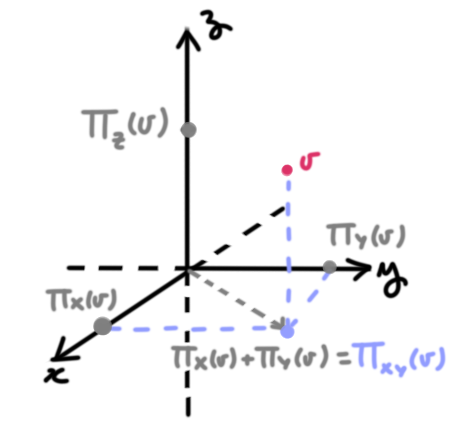
\includegraphics[scale=1.7]{31Julio_1} 
\end{figure}	



\QEDB
\vspace{0.2cm}


\begin{prop} \label{prop: elemento de la suma ortogonal de subespacios}
Si $\{ V_{j} \}_{j=1}^{n}$ es una familia de subespacios 
cerrados
ortogonales dos a dos
y $v \in \ameboxplus_{j =1 }^{n} V_{j}$, entonces los (únicos) elementos
de los espacios $V_{j}$ que sumados son iguales a $v$
son las proyecciones de $v$ sobre estos:

\[
v = \suma{j=1}{n}{ \Pi_{V_{j}}(v)}.
\]
\end{prop}
\noindent
\textbf{Demostración.}
Sea $\cali{B}$ una BON para la suma directa; por el lema 
\ref{lema: BONs de sumas ortogonales}, sabemos que,
para cada $j$,
\[
\cali{B}_{j}:= \cali{B} \cap V_{j}
\]
es una BON para $V_{j}$.

Por ser la suma de estos espacios directa, sabemos
que existen únicos $v_{j} \in V_{j}$ tales que
\[
v=v_{1} + \cdots + v_{n}.
\]
Por el \TODO{THM 4.13, Conway},

\begin{equation}
\label{eq 1:prop elemento de la suma ortogonal de subespacios}
v_{j}= \suma{}{}{\{ <v_{j},e> | e \in \cali{B}_{j}  \}}.
\end{equation}


Observe ahora que
\begin{equation}
\label{eq 2:prop elemento de la suma ortogonal de subespacios}
\suma{}{}{\{ <v_{j},e> | e \in \cali{B}_{j}  \}}=
\suma{}{}{\{ <v,e> | e \in \cali{B}_{j}  \}};
\end{equation}

en efecto, 
esto se deduce de inmediato del notar que,
para toda $e \in \cali{B}_{j}$,
\begin{align*}
<v, e> = & <v_{1} + \cdots + v_{n}, e> \\
= & <v_{1}, e> + \cdots + <v_{n}, e> \\
= & <v_{j}, e> 
\end{align*}
(dándose la última igualdad por ser $e \in V_{j} \subseteq V_{i}^{\perp}$
ortogonal a todos los $v_{i} \in V_{i}$ con $i \neq j$.) \\

Ahora bien, según el corolario \TODO{Ex. 13 conway},
\begin{equation}
\label{eq 3:prop elemento de la suma ortogonal de subespacios}
\suma{}{}{\{ <v,e> | e \in \cali{B}_{j}  \}}= \Pi_{V_{j}}(v).
\end{equation}

Juntando lo establecido en las igualdades
\eqref{eq 1:prop elemento de la suma ortogonal de subespacios},
\eqref{eq 2:prop elemento de la suma ortogonal de subespacios} y
\eqref{eq 3:prop elemento de la suma ortogonal de subespacios}
llegamos, como queríamos, a que
$v_{j}= \Pi_{V_{j}}(v).$

\QEDB
\vspace{0.2cm}


\begin{defi}
Si $\{ V_{j} \}_{j \in \IN}$ es una familia 
numerable de subespacios cerrados
de $V$ ortogonales dos a dos, definimos
a $\ameboxplus_{j \in \Delta} V_{j}$ como el siguiente
subespacio cerrado de $V$:
\begin{align*}
\ameboxplus_{j \in \IN} V_{j} := & \hspace{0.2cm}
\overline{\{ v_{1}+ \ldots + v_{n} :
n \in \IN, v_{j} \in V_{j}
\hspace{0.4cm} \text{para toda} \hspace{0.2cm} j \}} \\
= & \hspace{0.2cm} \overline{\union{n \in \IN}{}{\suma{j=1}{n}{V_{j}}}}
= \hspace{0.2cm} \overline{\union{n \in \IN}{}{\ameboxplus_{j=1}^{n} V_{j}}} .
\end{align*}
\end{defi}


\begin{prop} \label{prop: caracterizacion suma infinita de subespacios ortogonales} 
Con los elementos de la definición anterior,
$ v \in \ameboxplus_{j \in \IN} V_{j} $
si y sólo si existe $(v_{j})_{j \in \IN}$ 
elemento del producto cartesiano de la familia 
$\{ V_{j} \}_{j \in \IN}$
\footnote{i.e. una sucesión
de $V$, con $v_{j} \in V_{j}$ para toda $j$}
tal que 
\begin{itemize}
\item $v = \suma{j=1}{\infty}{v_{j}}$ y
\item $\suma{j=1}{\infty}{|| v_{j} ||^{2}}< \infty $.
\end{itemize}
De hecho, $(v_{j})_{j \in \IN}$ es el único elemento
del producto cartesiano de la familia cuya sucesión de
sumas parciales converge a $v$. Además, se tiene la igualdad
$|| v ||^{2}= \suma{j=1}{\infty}{|| v_{j} ||^{2}} $.
\end{prop}
\noindent
\textbf{Demostración.}
\begin{itemize} 
\item[$\Leftarrow$)] Es claro cómo el que exista una tal
sucesión $(v_{j})_{j \in \IN}$ ya implica que $v$ sea
elemento de $ \ameboxplus_{j \in \IN} V_{j} $ pues,
dado $\epsilon >0$ cualquiera, por definición de convergencia 
de series existe un $n \in \IN$ tal que
\[
| v - \suma{j=1}{n}{v_{j}} | < \epsilon . 
\]
\item[$\Rightarrow$)]  Sea $v \in \ameboxplus_{j \in \IN} V_{j} $;\\
(Existencia)
Si mostramos que
\[
v = \limite{J \rightarrow \infty}{v_{J}}, \hspace{0.4cm}
\text{donde} \hspace{0.2cm} v_{J}:= \Pi_{\ameboxplus_{j =1}^{J} V_{j}}(v),
\]
puesto que según el lema \ref{lema: proyección sobre la suma ortogonal}
$v_{J}= \suma{j=1}{J}{\Pi_{V_{j}}(v)}$,
tendremos que el elemento \[
\left( \Pi_{V_{j}(v)} \right)_{j \in \IN}
\]
del producto cartesiano de la familia
es tal que
\[
\suma{j=1}{\infty}{\Pi_{V_{j}}(v)}
= \lim_{J \rightarrow \infty} \suma{j=1}{J}{\Pi_{V_{j}}(v)}
= \limite{J \rightarrow \infty}{v_{J}}=v.
\]


Supongamos pues que existe $\epsilon >0$
para el que no sea posible hallar un $J>0$ tal que
$| v - v_{J} | < \epsilon $. Por definición del espacio 
$\ameboxplus_{j \in \IN} V_{j}$, sí que existen $J>0$
y $v_{j} \in V_{j}$, con $1 \leq j \leq J$ 
tales que $|v - \suma{i=1}{J}{v_{i}}| < \epsilon $; hemos
hallado así al elemento $\suma{i=1}{J}{v_{i}}$ de 
$\ameboxplus_{j =1}^{J} V_{j}$
tal que
\[
|v - \suma{i=1}{J}{v_{i}} | < \epsilon \leq |v - v_{J}| 
= |v - \Pi_{\ameboxplus_{j =1}^{J} V_{j}}(v) |,
\]

contradiciendo la definición del vector 
$\Pi_{\ameboxplus_{j =1}^{J} V_{j}}(v)$.



(Unicidad) Sea ahora
$(a_{j})$ elemento del producto cartesiano tal que $\suma{j=1}{\infty}{a_{j}}=0$.
Tenemos la siguiente cadena de igualdades;
\begin{align*}
0 = <0,0> = & < \suma{j=1}{\infty}{a_{j}} , \suma{j=1}{\infty}{a_{j}}  > \\
= & < \limite{n \rightarrow \infty}{\suma{j=1}{n}{a_{j}}},
\limite{n \rightarrow \infty}{\suma{j=1}{n}{a_{j}}}> \\
\text{(por proposición \ref{prop: continuidad del producto punto})}
= & \limite{n \rightarrow \infty}{ \langle \suma{j=1}{n}{a_{j}}  ,
\suma{j=1}{n}{a_{j}} \rangle }  \\
\text{(por ortogonalidad)}= & \limite{n \rightarrow \infty}{\suma{i=1}{n}{|| a_{i}||^{2}}};
\end{align*}
deducimos a partir de ella que la norma de cada $a_{j}$ es cero;
así, el suponer $\suma{j=1}{\infty}{a_{j}}=0$ implica la igualdad
a cero de cada
$a_{j}=0$.  De esto deducimos que, para todo 
$v \in \ameboxplus_{j \in \IN} V_{j}$, si $(v_{j})$ y $(w_{j})$
son dos
elementos del producto cartesiano para los que
$\suma{j=1}{\infty}{v_{j}}=v = \suma{j=1}{\infty}{w_{j}}$,
entonces
\[
\suma{i=1}{\infty}{(v_{j}-w_{j})}= 
\suma{j=1}{\infty}{v_{j}} - \suma{j=1}{\infty}{w_{j}} = v-v=0,
\]
de donde $v_{j}=w_{j}$. \\

Mostremos por último que $|| v ||^{2} = \suma{i=1}{\infty}{|| v_{i} ||^{2}} $.
Por la bilinealidad del producto punto y
y la ortogonalidad de los subespacios, para toda $n \in \IN$
\[
< v_{1}+ \ldots + v_{n} , v_{1}+ \ldots + v_{n}  > =
< v_{1} , v_{1} > + \ldots + < v_{n} , v_{n} >,
\]
luego,
\begin{align*}
\suma{i=1}{\infty}{||v_{i}||^{2}} = &
\limite{n \rightarrow \infty}{\suma{i=1}{n}{||v_{i}||^{2}}} \\
= & \limite{n \rightarrow \infty}{\langle 
\suma{i=1}{n}{v_{i}} , \suma{i=1}{n}{v_{i}} \rangle };
\end{align*}
por la continuidad establecida en la 
proposición \ref{prop: continuidad del producto punto},
podemos continuar la cadena de igualdades como sigue:
\begin{align*}
\suma{i=1}{\infty}{||v_{i}||^{2}} = & \langle  \limite{n \rightarrow \infty}{\suma{i=1}{n}{v_{i}}} ,
 \limite{n \rightarrow \infty}{\suma{i=1}{n}{v_{i}}} \rangle \\
 & = < v , v > = ||v||^{2}.
\end{align*}
\end{itemize}
\QEDB
\vspace{0.2cm}
\newpage
\section{La transformada discreta de Fourier}
\label{sec: TDF}

En esta sección vamos a dar la definición usual de 
las bases de Fourier complejas y reales, que son
bases ortonormales de $\IC^{n}$ y de $\IR^{n}$ 
\marginnote{Incluimos este capítulo de teoría clásica
por completitud de este trabajo
y para fijar la notación. 
\cite{fourier1} y \cite{fourier2}
son referencias con mucha más información.}
de $\IC^{n}$
y una de $\IR^{n}$ (que llamaremos
``bases de Fourier complejas y reales''),
definidas ambas en términos de discretizaciones de
sinusoides de frecuencias enteras, y que son herramientas
clásicas para hacer lo que comúnmente se denomina
un \textbf{análisis espectral} de señales finitas.


Puesto que la definición de estas herramientas requiere
de algunas nociones del análisis complejo (en particular, de la
definición de la exponencial compleja y de las raíces $n-$ésimas
de la unidad), damos brevemente algunas definiciones y resultados
necesarios para definir las bases de Fourier.


\subsection{La exponencial compleja y raíces $n-$ésimas de la unidad}


La definición de la función exponencial compleja 
tiene diversas motivaciones
(puede consultar algunas de estas en 
\cite{marsden}). Nosotros sólo
damos la definición de esta, así como algunas propiedades
de ella que se usarán en lo que sigue.

\begin{defi}
\label{def: exponencial compleja}
Si $y \in \IR$, entonces por $exp(iy)$ denotamos al número
complejo de módulo uno y argumento $y$, es decir,
\begin{equation}
\label{eq: exponencial 1}
exp(iy) := cos(y) + i sen(y).
\end{equation}
Para todo número complejo $z = a+bi$, definimos 
$exp(z)$ como sigue:
\begin{equation}
\label{eq: exponencial 2}
exp(z) := e^{x}(cos(y) + i sen(y)).
\end{equation}
\end{defi}

\begin{prop}
\label{prop: propiedades exp compleja}
(\textbf{Algunas propiedades de la exponencial compleja}) 
Sean $z_{1}, z_{2} \in \IC$, $\omega \in \IZ$.
	\begin{itemize}
	\item $\frac{exp(z_{1})}{exp(z_{2})} = exp(z_{1} - z_{2})$
	\item $exp(z_{1} + z_{2}) = exp(z_{1}) \cdot exp(z_{2})$
	\item $(exp(z_{1}))^{\omega} = exp(\omega z)$
	\item $exp(z) = 1$ si y sólo si $z= 2K \pi i$ para algún $K \in \IZ$ 
	\item para todo $y \in \IR$, 
	\begin{equation}
	\label{eq: coseno exponenciales}
	cos(y) = \frac{exp(iy)+exp(-iy)}{2}
	\end{equation}
	y
	\begin{equation}
	\label{eq: seno exponenciales}
	sen(y) = \frac{exp(iy)-exp(-iy)}{2i}.
	\end{equation}
	\end{itemize}
\end{prop}

\begin{defi}
\label{defi: raices n esimas de la unidad}
Sea $n \in \IN$. A las $n$ raíces complejas del polinomio
$p_{n}(t)= t^{n}-1 \in \IC[t]$ 
se les denominará las \textbf{raíces $n-$ésimas de la unidad.}
\end{defi}


Las raíces $n-$ésimas de la unidad son pues los números complejos
tales que, elevados a la potencia $n$, son iguales a 1; según el 
teorema fundamental
del álgebra \ref{teo: fundamental del algebra}, sí hay números complejos
que satisfacen la definición \ref{defi: raices n esimas de la unidad}, y además
son a lo más $n$. Es fácil establecer, como hacemos a continuación, 
fórmulas explícitas para estos números, que de hecho son exactamente $n$.

\begin{prop}
Sea $n \in \IN$, $n \geq 2$. Hay exactamente $n$ raíces $n-$ésimas de la
unidad, y estas son los números complejos
 	\begin{equation}
	\label{eq3: 8ab}
	z_{n, \omega} : = exp \left( \frac{2 \pi i }{n} \omega
	\right), \hspace*{0.2cm} \textit{con} 
	\hspace*{0.2cm} \omega \in \{0, 1, \ldots, n-1 \}.
	\end{equation}
	
\end{prop}
\noindent
\textbf{Demostración.}
Por las propiedades expresadas en la proposición
\ref{prop: propiedades exp compleja}, es fácil ver que 
$z_{n,1} :=  exp \left( \frac{2 \pi i }{n} \right)$ es raíz $n-$ésima
de la unidad, pues
\[
(z_{n,1})^{n} = exp(2 \pi i ) = 1.
\]
Además, para todo $\omega \in \{ 0, \cdots , n-1 \}$, el número
\[
z_{n, \omega} : = (z_{n,1})^{\omega} = exp \left( \frac{2 \pi i }{n} \omega \right)
\]
también es es raíz $n-$ésima de la unidad, ya que

\[
(z_{n, \omega})^{n} = ((z_{n,1})^{\omega} )^{n} = 
((z_{n,1})^{n} )^{\omega} = 1^{\omega}=1. 
\]
Note ahora que los $n$ números complejos $z_{n, \omega}$ son todos 
distintos entre sí, pues si $\omega_{1}$ y $\omega_{2}$ son enteros
entre $0$ y $n-1$ tales que $z_{n, \omega_{1}} = z_{n, \omega_{2}}$,
o sea, tales que 
$exp \left( \frac{2 \pi i }{n} \omega_{1} \right) = 
exp \left( \frac{2 \pi i }{n} \omega_{1} \right)$, entonces, según el primer
punto de la proposición \ref{prop: propiedades exp compleja},
$1 = exp \left( \frac{2 \pi i }{n} (\omega_{1}-\omega_{2}) \right)$, luego, 
según el cuarto punto de esta misma proposición, $\frac{\omega_{1}-\omega_{2}}{n}$
es entero, o sea, $n$ divide a $\omega_{1}-\omega_{2}$; por el rango de 
$\omega_{1}$ y $\omega_{2}$, esto sólo ocurre si $\omega_{1}-\omega_{2}$ es
cero, o sea, si $\omega_{1}$ y $\omega_{2}$
son iguales.
\QEDB
\vspace{0.2cm}

\begin{figure}[H]
	\sidecaption{
	Para construir gráficamente a las raíces $n-$ésimas de la
	unidad, se debe dividir, a partir del punto $(0,1)$, a la
	circunferencia unitaria en $n$ partes iguales. Según esta construcción
	y la interpretación geométrica de la multiplicación compleja, es claro
	que multiplicando a $z_{n,1}$ consigo mismo se obtienen a
	todas las demás raíces $n-$ésimas.
	\label{fig: raices unidad}
	}
	\centering
	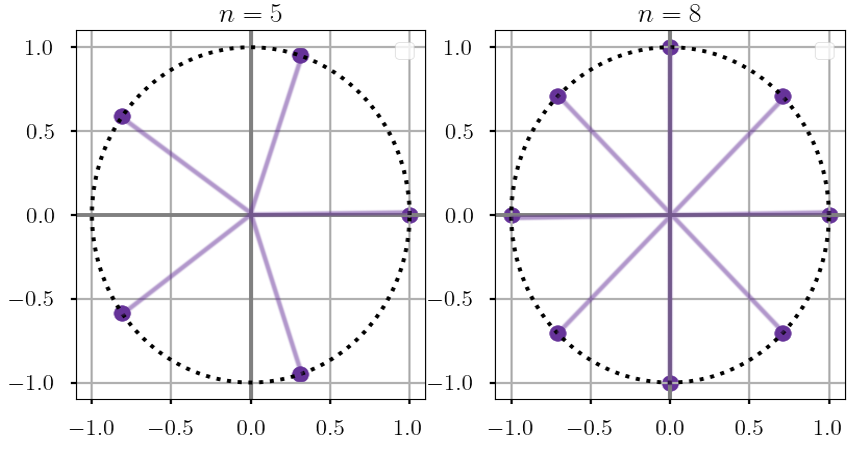
\includegraphics[scale=0.53]{raices_unidad} 
\end{figure}	


\subsection{La transformada discreta de Fourier}

Ya tenemos todo lo necesario para definir a la base
de Fourier compleja de la que hablamos al inicio.
\marginnote{El producto punto que estamos
considerando en el $\IC-$espacio
vectorial $\IC^{n}$ es el que definimos
en \eqref{eq: producto punto Cn}, y el del
$\IR-$espacio vectorial $\IR^{n}$ es el definido en 
\eqref{eq: producto punto Rn}.}

\begin{prop}
\label{prop: construccion Bn}
Sea $n \in \IN$. El conjunto

\begin{equation}
\label{eq2: 8ab}
\cali{B}_{n} : = \left\{
e_{n,\omega} = \left(
\frac{1}{\sqrt{n}} exp \left(
2 \pi i \omega \frac{m}{n}
\right)
\right)_{0 \leq m \leq n-1}
: \hspace{0.2cm} 0 \leq \omega \leq n-1
 \right\}
\end{equation}
es una base ortonormal del $\IC-$espacio
vectorial $\IC^{n}$.
\end{prop}

\noindent
\textbf{Demostración.}
Calculemos el producto punto de dos elementos
$e_{n,\omega_{1}}$ y $e_{n,\omega_{2}}$ del conjunto \eqref{eq2: 8ab};
si $\omega := \omega_{1}-\omega_{2}$,
\begin{align*}
\langle e_{n,w_{1}}, e_{n,w_{2}} \rangle = &
\frac{1}{n}
\suma{m=0}{n-1}{exp \left( 2 \pi i \frac{m}{n} \omega_{1} \right)
\cdot \overline{ exp \left( 2 \pi i \frac{m}{n} \omega_{2} \right) }} \\
= & \frac{1}{n}
\suma{m=0}{n-1}{\left( 2 \pi i \frac{m}{n} (\omega_{1}-\omega_{2}) \right)} \\
= & \frac{1}{n}\suma{m=0}{n-1}{exp\left( 2 \pi i \frac{\omega}{n} m \right)} \\
= & \frac{1}{n}\suma{m=0}{n-1}{exp\left( 2 \pi i \frac{\omega}{n}  \right)^{m}} \\
= & \frac{1}{n}\suma{m=0}{n-1}{(z_{n, \omega})^{m}};
\end{align*}

\noindent
esta última es una suma geométrica. 
\begin{itemize}
	\item Si $\omega_{1} \neq \omega_{2}$, entonces $n$ no puede dividir 
	a $\omega = \omega_{1}-\omega_{2}$ (pues, por el rango en el que se encuentran
	$\omega_{1}$ y $\omega_{2}$, $w \in [-(n-1), n-1]$, y el único múltiplo
	de $n$ en este intervalo es cero), luego, $z_{n, \omega} \neq 1$.
	En este caso se tiene entonces que 
	\[
	\langle e_{n,w_{1}}, e_{n,w_{2}} \rangle = 
	\frac{1}{n}\suma{m=0}{n-1}{(z_{n, \omega})^{m}}
	= \frac{1}{n} \cdot \frac{(z_{n, \omega})^{n}-1}{z_{n, \omega}-1}=
	\frac{1}{n} \cdot \frac{1-1}{z_{n, \omega}-1}=0.
	\]
	
	\item Si $\omega_{1} = \omega_{2}$, entonces $\omega = 0$, y
	\[
	\langle e_{n,w_{1}}, e_{n,w_{2}} \rangle = 
	\frac{1}{n}\suma{m=0}{n-1}{(z_{n, 0})^{m}}
	= \frac{1}{n}\suma{m=0}{n-1}{1} = \frac{1}{n} \cdot n = 1.
	\]
\end{itemize}

Demostramos así que los elementos de $\cali{B}_{n}$
tienen norma uno y que además
son ortogonales
dos a dos, luego, $\cali{B}_{n}$ es un subconjunto l.i. 
de $\IC^{n}$; como $\IC^{n}$ es un $\IC-$espacio vectorial de 
dimensión $n$, concluimos lo deseado.
\QEDB
\vspace{0.2cm}

Por ser \eqref{eq2: 8ab} una BON de $\IC^{n}$, siempre es
posible expresar a un vector $x = (x_{m})_{0 \leq m \leq n-1} \in \IC^{n}$
como combinación lineal de los elementos de \eqref{eq2: 8ab}
y además los coeficientes están dados por los productos punto
de $x$ y los elementos de \eqref{eq2: 8ab}
(c.f. nota \ref{nota: sobre la identidad de parseval}).

\begin{defi}
Sean $n \in \IN$, $x = (x_{m})_{m=0}^{n-1} \in \IC^{n}$
una señal compleja de longitud $n$.
Sea $\cali{B}_{n}$ la base de $\IC^{n}$ definida en 
la proposición \ref{prop: construccion Bn}. \\

A la función $f_{x}: \{ 0, 1, \ldots, n-1 \} 
\rightarrow \IC^{n}$ que a cada
frecuencia $\omega \in \{ 0, 1, \ldots, n-1 \} $
le asocia el coeficiente de $x$ respecto 
al elemento $e_{n, \omega}$ de la base
$\cali{B}_{n}$, o sea, la función definida como
\begin{equation}
\label{eq: TDF}
f_{x}(\omega) = X_{\omega} := 
\frac{1}{\sqrt{n}} \suma{m=0}{n-1}{x_{m} exp \left(
2 \pi i \omega \frac{m}{n}
\right)}
\end{equation}
le llamaremos la 
\textbf{transformada discreta de Fourier de $x$}.
Muchas veces identificamos a tal transformada
con el vector
$X := (X_{\omega})_{\omega = 0}^{n-1}$, que 
no es más que la representación 
de $x = (x_{m})_{m=0}^{n-1}$ respecto a la 
base de frecuencias $\cali{B}_{n}$.
\end{defi}

\marginnote{Por sus siglas en inglés, a la transformada discreta
de Fourier también se le denomina ``TDF''.}


\begin{comment}
{\Huge{\textcolor{red}{TDF}}} 

{\Huge{\textcolor{red}{Dominio: tiempo}}} 


{\Huge{\textcolor{red}{Dominio: frecuencia}}}

{\Huge{ $x = (x_{m})_{0 \leq m \leq n-1}$ }}

{\Huge{ $\langle x, e_{\omega} \rangle$, $0 \leq \omega \leq n-1 $ }}

\end{comment}

Calcular entonces la transformada discreta de Fourier
de $x$ consiste en calcular a los productos
punto $\langle x, e_{n,\omega} \rangle $, que son

\begin{align*}
X_{\omega} := \langle x, e_{n,\omega} \rangle = & 
\frac{1}{\sqrt{n}} \suma{m=0}{n-1}{x_{m} exp \left(
2 \pi i \omega \frac{m}{n}
\right)} \\
= & 
\frac{1}{\sqrt{n}} \suma{m=0}{n-1}{x_{m} 
\left(
exp \left( \frac{2 \pi i }{n} \omega
\right) \right)^{m}} \\
= & A_{x}(z_{n, \omega}),
\end{align*}


\noindent
donde $z_{n, \omega}$ es como en \eqref{eq3: 8ab} y 
$A_{x} = A_{x}(t) \in \IC[t]$ es el polinomio de 
coeficientes complejos definido 
a partir de $x$ como sigue:

	\begin{equation}
		\label{eq4: 8ab}
		A_{x}(t) := \suma{m=0}{n-1}{\frac{x_{m}}{\sqrt{n}} t }\in \IC[t];
	\end{equation}

\noindent
así, \textbf{calcular la transformada
discreta de Fourier de $x$ es lo mismo que evaluar al polinomio 
$A_{x}$ de grado a lo más $n-1$ definido en \eqref{eq4: 8ab} en todas las raíces
$n-$ésimas de la unidad.} 


\begin{nota}
Según este último párrafo, calcular transformadas discretas
de Fourier requiere de algoritmos eficientes para evaluar
polinomios en raíces $n-$ésimas de la unidad. Usando propiedades
de las raíces $n-$ésimas de la unidad (por ejemplo,
véase el lema 30.5 de \cite{algorithms}) 
es posible usar recursión para disminuir
el tiempo de cómputo. Al algoritmo estándar usado para
esto se le conoce como la \textbf{transformada rápida de 
Fourier} (abreviado como ``FFT'' por sus siglas en inglés);
puede consultar los detalles técnicos en el capítulo
30 de \cite{algorithms}.
\end{nota}

\begin{nota}
Se calcula fácilmente una fórmula para la 
inversa de la transformada discreta de Fourier 
$f_{x}$ de una señal $x$; si
se conoce la TDF $X = (X_{\omega})_{\omega=0}^{n-1}$
de una señal $x \in \IC^{n}$, pueden recuperarse sus coeficientes
respecto a la base canónica de $\IC^{n}$ (i.e. su representación
respecto al tiempo)
como sigue:
\begin{equation}
\label{eq: TDFI}
\forall \hspace{0.1cm} 0 \leq m \leq n-1:
\hspace{0.2cm}
x_{m} = \frac{1}{\sqrt{n}} 
\suma{k=0}{n-1}{
X_{k} exp \left( 
-2 \pi i k \frac{m}{n}
\right).
}
\end{equation}

En ocasiones, por transformada discreta de Fourier y su 
inversa se toman las opuestas a las que hemos definido aquí
(i.e. se pide el signo negativo en la exponencial 
para la TDF y se toma el signo positivo para la inversa); además,
se toman distintos factores de normalización
(por ejemplo, $1$ para la TDF y $\frac{1}{n}$ para la
inversa), c.f. \cite{TDFwiki}. Puede ver que fórmulas
para la TDF y su inversa son implementadas en el 
módulo \texttt{scipy.fft} de Python con las modificaciones descritas
antes (puede consultar la documentación de esta librería en
\cite{FFTscipy}).
\end{nota}

\begin{figure}[H]
\centering\captionsetup{format = hang}
	\begin{measuredfigure}
		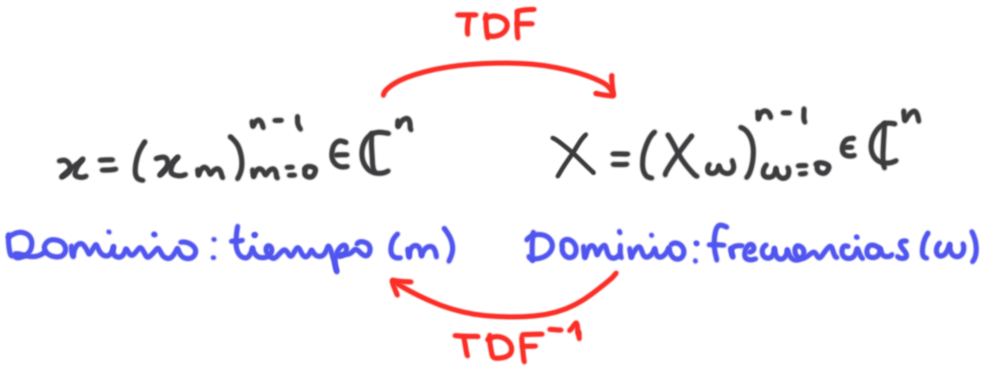
\includegraphics[scale=1.35]{tiempo_freq.png} 
		\caption{Usualmente uno representa a una señal discreta
		$x$ de dimensión $n$ con $n$ mediciones complejas; en este caso, el dominio
		de la representación es el tiempo. Pero
		también se puede representar unívocamente a $x$ con sus
		coeficientes respecto a la base de frecuencias 
		$\cali{B}_{n}$; en este caso, puesto que cada coeficiente da
		el peso que tiene la respectiva frecuencia para construir la 
		señal original $x$, decimos que el dominio de la representación
		es el de frecuencia. Las fórmulas para pasar de una
		representación a otra son \eqref{eq: TDF} y \eqref{eq: TDFI}.}
 	\end{measuredfigure}
\end{figure}


Al usar a $\cali{B}_{n}$ como sistema de representación en
$\IC^{n}$, lo que estamos haciendo es representar a
un $x = (x_{m})_{0 \leq m \leq n-1}$ como combinación
lineal de los vectores 

\[
e_{n,\omega} = \frac{1}{\sqrt{n}} \left( cos
\left( 2 \pi \omega \frac{m}{n} \right)
+ i sen \left( 2 \pi \omega \frac{m}{n}\right) \right)_{0\leq m \leq n-1},
\hspace{0.2cm} 0 \leq \omega \leq n-1;
\]
observe que las partes reales de las
entradas de $e_{n,\omega} \in \IC^{n}$ se obtienen de tomar $n$
muestras uniformes de la función 
$c_{\omega}(t) := \frac{1}{\sqrt{n}} cos (2 \pi \omega t)$ (o sea, de la función
coseno de amplitud $\frac{1}{\sqrt{n}}$, frecuencia $\omega$ y desfase $0$)
y, similarmente,
las partes imaginarias de las entradas se obtienen muestreando
uniformemente a la función 
$s_{\omega}(t) := \frac{1}{\sqrt{n}}  sin (2 \pi \omega t)$.

\begin{figure}[H]
	\sidecaption{
	Por ejemplo, si $n=5$, para construir al vector
	$e_{3}$ de la base $\cali{B}_{n}$ se muestrean uniformemente
	cosenos y senos de frecuencia $3$ como se muestra en la figura;
	los puntos rojos representan las partes reales de las entradas
	y los azules las imaginarias.
	\label{fig: construccion Bn}
	}
	\centering
	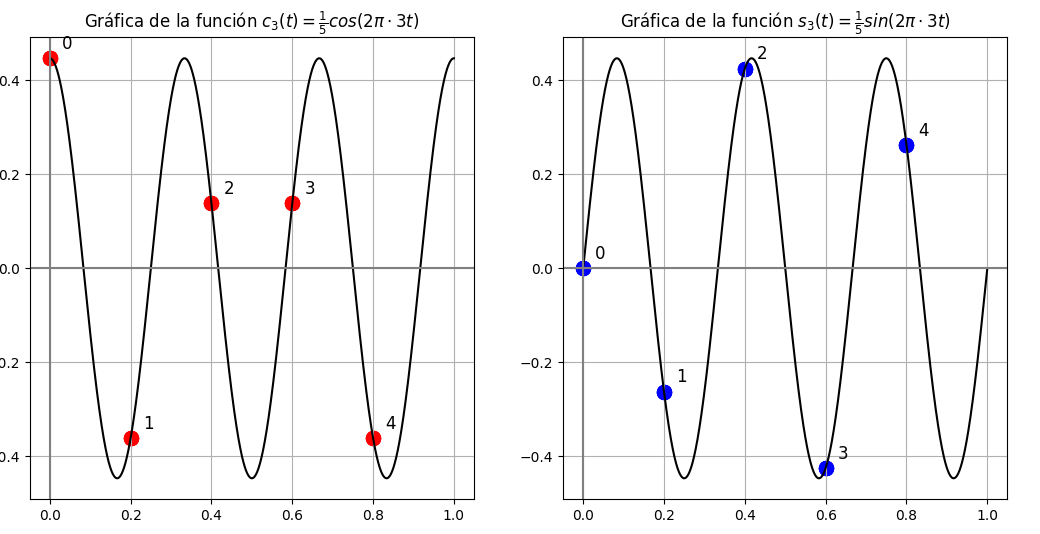
\includegraphics[scale=0.29]{construccion_Bn} 
\end{figure}	

Según esto, el vector $e_{n,\omega}$ se construye a partir
de funciones de frecuencia $\omega$; considerando esto
y el que $\cali{B}_{n}$ sea una BON de $\IC^{n}$ (luego, el
que se valga la identidad de Parseval,
c.f. nota \ref{nota: sobre la identidad de parseval}), tenemos que
la síntesis

\[
x = \suma{\omega=0}{n-1}{\langle x, e_{n,\omega} \rangle e_{n,\omega}}
\]

\noindent
es una expresión de $x$ en términos de vectores de frecuencia
$\omega$ y que los respectivos coeficientes 
$\langle x, e_{n,\omega} \rangle$ indican qué tanto 
contribuye la frecuencia $\omega$ para construir a $x$.

Es por eso que al proceso de considerar representaciones
de señales complejas finitas respecto a las bases de Fourier
se le conoce como  
\textbf{realizar un análisis espectral.}


\subsection{Versión real de la TDF}

En el caso en el que todas las entradas de un vector
$x = (x_{m})_{0 \leq m \leq n-1}$ sean reales, se puede definir
una base ortonormal de $\IR^{n}$, 
análoga a la BON $\cali{B}_{n}$ de $\IC^{n}$ construida en 
\ref{prop: construccion Bn},
a partir de muestreos uniformes
de sinusoides de frecuencias enteras.

\begin{prop}
\label{prop: base de fourier version real}
Sean $n \in \IN$ mayor a uno, $M = \lceil \frac{n}{2} \rceil$.
Definimos a los vectores de $\IR^{n}$

\[
c_{n, 0}= \left( \sqrt{\frac{1}{n}} cos
	\left(2 \pi \cdot 0 \frac{m}{n}
	\right) \right)_{m=0}^{n-1} = 
	\left( \frac{1}{\sqrt{n}}, \cdots, \frac{1}{\sqrt{n}} \right),
\]

	\begin{equation}
	\label{eq0: 10ab}
	c_{n, \omega} := \left( \sqrt{\frac{2}{n}} cos
	\left(2 \pi \omega \frac{m}{n}
	\right) \right)_{m=0}^{n-1},
	\hspace{0.2cm} 1 \leq \omega \leq M-1
	\end{equation}
	
	\begin{equation}
	\label{eq0: 4May}
	s_{n, \omega} := \left( \sqrt{\frac{2}{n}} sin
	\left(2 \pi \omega \frac{m}{n}
	\right) \right)_{m=0}^{n-1},
	\hspace{0.2cm} 1 \leq \omega \leq M-1
	\end{equation}
	
y, en el caso en que n sea par, definimos también
al vector

	\[
c_{n, M}= \left( \sqrt{\frac{1}{n}} cos
	\left(2 \pi \cdot M \frac{m}{n}
	\right) \right)_{0 \leq m \leq n-1} = 
	\left( \frac{(-1)^{m}}{\sqrt{n}} \right)_{m=0}^{n-1}.
\]

El subconjunto $\cali{F}_{n}$ de $\IR^{n}$ definido como

	\begin{itemize}
	\item $\cali{F}_{n} : = \{ c_{n,0}, c_{n,1}, s_{n,1},
	\ldots , c_{n,M-1}, s_{n,M-1}, c_{n,M} \}$ si $n$ es par
	(o sea, si $n=2M$), y como
	\item $\cali{F}_{n} : = \{ c_{n,0}, c_{n,1}, s_{n,1},
	\ldots , c_{n,M-1}, s_{n,M-1} \}$ si $n$ es impar
	(o sea, si $n=2M-1$)
	\end{itemize}
	
es una base ortonormal del $\IR-$espacio vectorial $\IR^{n}$.
\end{prop}

\noindent
\textbf{Demostración.}
Supongamos $n$ par. Si $0 \leq \omega_{1}, \omega_{2} \leq M$
son enteros, entonces
$\omega_{1} + \omega_{2}$ sólo es divisible por $n$ si ambos números
son iguales a $M$. Si suponemos a $\omega_{1}$ y $\omega_{2}$ distintos, 
entonces

\begin{align*}
\langle c_{n, \omega_{1}} , c_{n, \omega_{2}} \rangle = &
\frac{1}{n} \suma{m=0}{n-1}{cos \left(2 \pi \omega_{1} \frac{m}{n} \right) \cdot 
cos \left(2 \pi \omega_{2} \frac{m}{n} \right)} \\
= &\frac{1}{2n} \left(
cos \left(2 \pi (\omega_{1} + \omega_{2}) \frac{m}{n} \right) +
cos \left(2 \pi (\omega_{1} - \omega_{2}) \frac{m}{n} \right)
\right) \\
= & \frac{1}{4n} (
\suma{m=0}{n-1}{
(exp(2 \pi m(\omega_{1}+\omega_{2})i/n) +
exp(-2 \pi m(\omega_{1}+\omega_{2})i) } \\
&  + exp(2 \pi m(\omega_{1}-\omega_{2})i/n) +
exp(-2 \pi m(\omega_{1}-\omega_{2})i)) )\\
\textit{(suma geométrica)} = & 
\frac{exp(2 \pi i (\omega_{1}+\omega_{2}))-1}{4n (exp(2 \pi i (\omega_{1}+\omega_{2})/n)-1)} +
\frac{exp(- 2 \pi i (\omega_{1}+\omega_{2}))-1}{4n (exp(-2 \pi i (\omega_{1}+\omega_{2})/n)-1)}
\\
& + 
\frac{exp(2 \pi i (\omega_{1}-\omega_{2}))-1}{4n (exp(2 \pi i (\omega_{1}-\omega_{2})/n)-1)} +
\frac{exp(- 2 \pi i (\omega_{1}-\omega_{2}))-1}{4n (exp(-2 \pi i (\omega_{1}-\omega_{2})/n)-1)};
\\
\end{align*}

\noindent
puesto que $\omega_{1}+\omega_{2}$ y $\omega_{1}-\omega_{2}$
son ambos enteros, según la proposición 
\ref{prop: propiedades exp compleja} las exponenciales de los numeradores
de esta última expresión son todas iguales a uno, luego, 
$\langle c_{n, \omega_{1}} , c_{n, \omega_{2}} \rangle  =0$. 


Con argumentos similares se prueba 
que todos los elementos de $\cali{F}_{n}$ tienen norma uno, así como
la ortogonalidad entre dos elementos
distintos del conjunto $\cali{F}_{n}$, por lo tanto, la independencia lineal de
este conjunto, luego, el que $\cali{F}_{n}$ sea base 
(ortonormal) de $\IR^{n}$.


\QEDB
\vspace{0.2cm}



\begin{defi}
Sea $n \in \IN$, $n \geq 2$. Llamaremos a la BON
$\cali{F}_{n}$ de $\IR^{n}$ definida en \ref{prop: base de fourier version real}
la \textbf{base de Fourier real de dimensión $n$}.
\end{defi}

\begin{nota}
\label{nota: frecuencias en las bases de fourier}
Observe que $\cali{F}_{n}$, a diferencia de $\cali{B}_{n} \subseteq \IC^{n}$, 
considera frecuencias enteras no mayores a $M := \lceil \frac{n}{2} \rceil$
(cuando $n$ es par) o a $M-1$ (cuando $n$ es impar), mientras que
en $\cali{B}_{n}$ se consideran las frecuencias enteras entre $0$
y $n-1$ (inclusivo); así, si decidimos representar
a una señal $x \in \IR^{n}$ en base a $\cali{F}_{n} \subseteq \IR^{n}$
y no en base a $\cali{B}_{n} \subseteq \IC^{n}$, sintetizaremos a $x$
respecto a frecuencias enteras acotadas por $M$ o por $M-1$ 
(dependiendo de la paridad de $n$), y no respecto a frecuencias
menores a $n$.
\end{nota}

\begin{ejemplo}
\label{ej: DFT1}
Consideremos a la señal 
\begin{equation}
\label{eq2: 10ab}
x=(-0.5,-8,-5.3,15,-0.3,6,4) \in \IR^{7}.
\end{equation}

Según la construcción de $\cali{F}_{7}$ (c.f. 
proposición \ref{prop: base de fourier version real}),
una expresión de $x$ respecto a $\cali{F}_{7}$ 
es una síntesis de $x$ a partir de señales 
de frecuencias $\omega = 0,1,2,3$. En la imagen de abajo
se muestran los coeficientes de $x$ respecto a $\cali{F}_{7}$.

\begin{figure}[H]
	\sidecaption{
	Se muestran la gráfica de $x$ junto con la gráfica de los
	coeficientes de $x$ respecto a la BON $\cali{F}_{7}$. Observe 
	que, por definición, sólo un vector de $\cali{F}_{7}$ tiene frecuencia
	cero (i.e. es constante), mientras que para las otras frecuencias
	tenemos dos vectores de la misma frecuencia, uno construido a partir de un 			
	coseno y otro a partir de un seno.
	\label{fig: ejFrecuencia 1}
	}
	\centering
	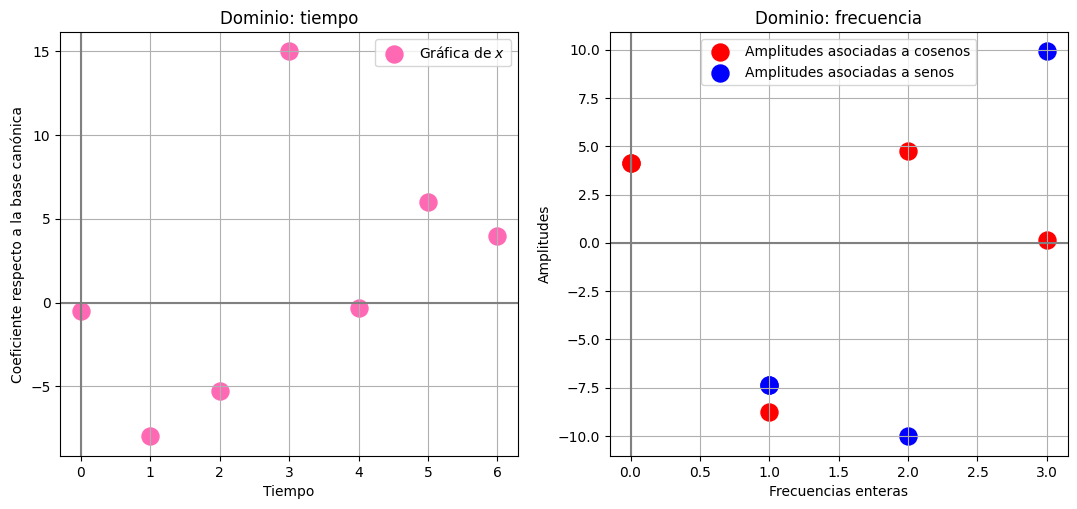
\includegraphics[scale=0.4]{ejFrecuencia_1} 
\end{figure}	

Redondeando los coeficientes, 
se tiene la siguiente descomposición de $x$;

\begin{equation}
\label{eq: analisis x TDF}
x = 4.12 c_{7,0} - 8.76c_{7,1} -7.35s_{7,1}+
4.77c_{7,2}-10s_{7,2}+0.14c_{7,3}+9.91s_{7,3}.
\end{equation}

\noindent
A continuación mostramos las gráficas
de los sinusoides que fueron discretizados
para obtener los vectores de frecuencia
$0,1,2$ y $3$ en los que descompusimos a $x$.

\begin{figure}[H]
	\sidecaption{
	Aporte de frecuencia $0$.
	\label{fig: ejFrecuencia 2}
	}
	\centering
	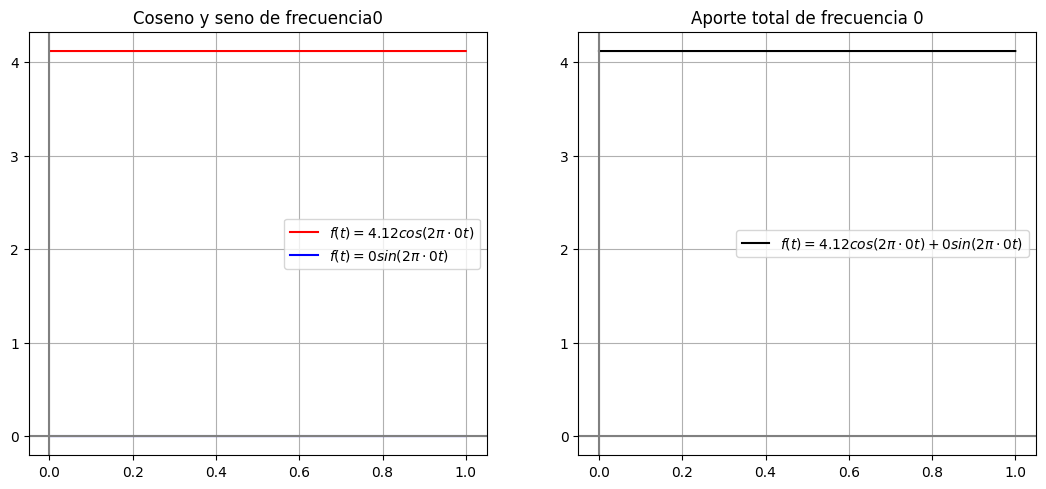
\includegraphics[scale=0.4]{ejFrecuencia_2} 
\end{figure}	

\begin{figure}[H]
	\sidecaption{
	Aporte de frecuencia $1$.
	\label{fig: ejFrecuencia 3}
	}
	\centering
	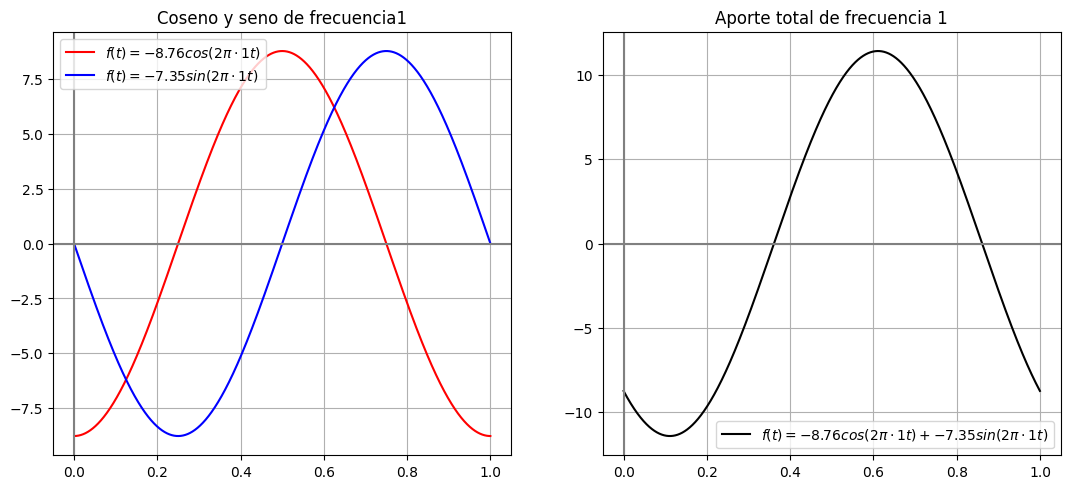
\includegraphics[scale=0.4]{ejFrecuencia_3} 
\end{figure}	

\begin{figure}[H]
	\sidecaption{
	Aporte de frecuencia $2$.
	\label{fig: ejFrecuencia 4}
	}
	\centering
	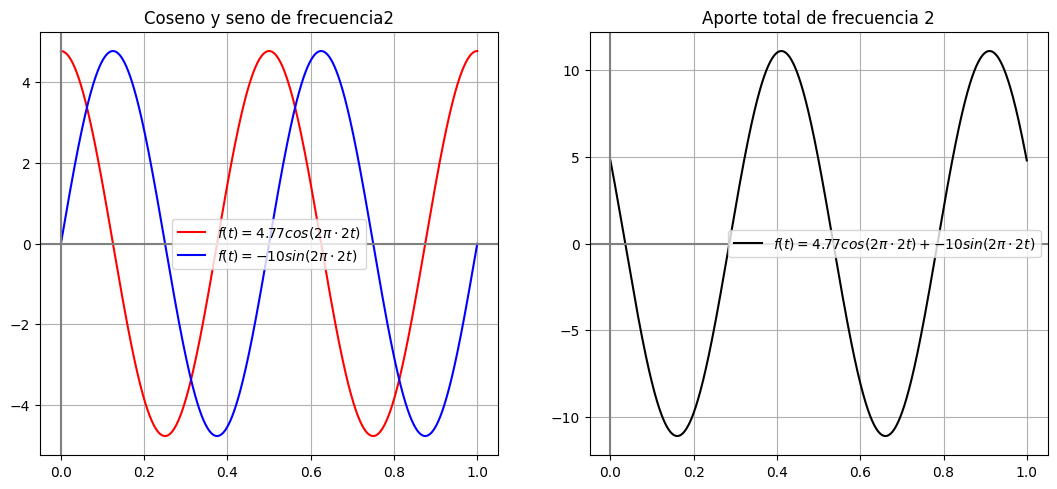
\includegraphics[scale=0.4]{ejFrecuencia_4} 
\end{figure}	


\begin{figure}[H]
	\sidecaption{
	Aporte de frecuencia $3$.
	\label{fig: ejFrecuencia 5}
	}
	\centering
	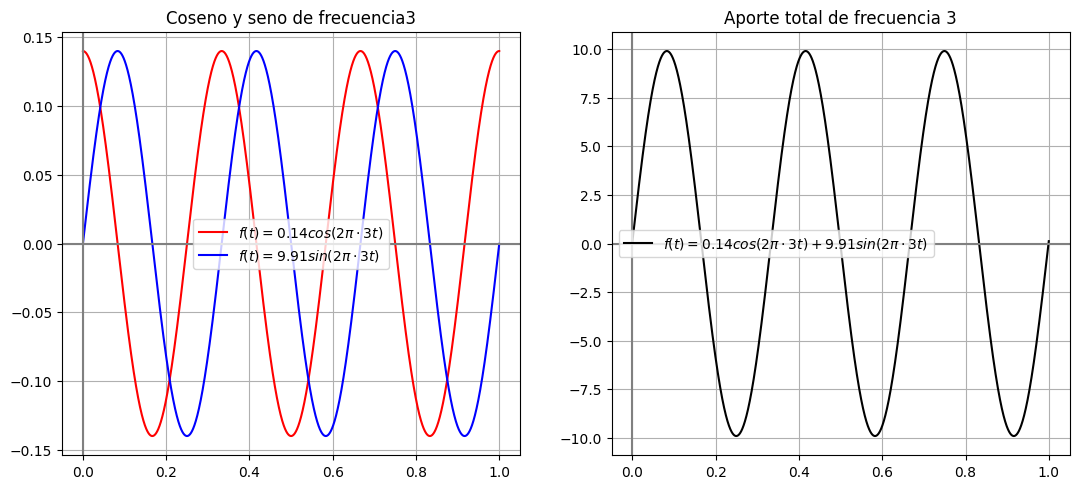
\includegraphics[scale=0.4]{ejFrecuencia_5} 
\end{figure}	

Sumando todas las gráficas de la derecha, obviamente
obtenemos una función de cosenos y senos tal que,
del muestrearla uniformemente en $[0,1]$, resulta
el vector $x$ \eqref{eq2: 10ab}.

\begin{figure}[H]
	\sidecaption{
	En morado se muestra la gráfica de la función suma
	de las gráficas derechas en las figuras anteriores.
	\label{fig: ejFrecuencia 6}
	}
	\centering
	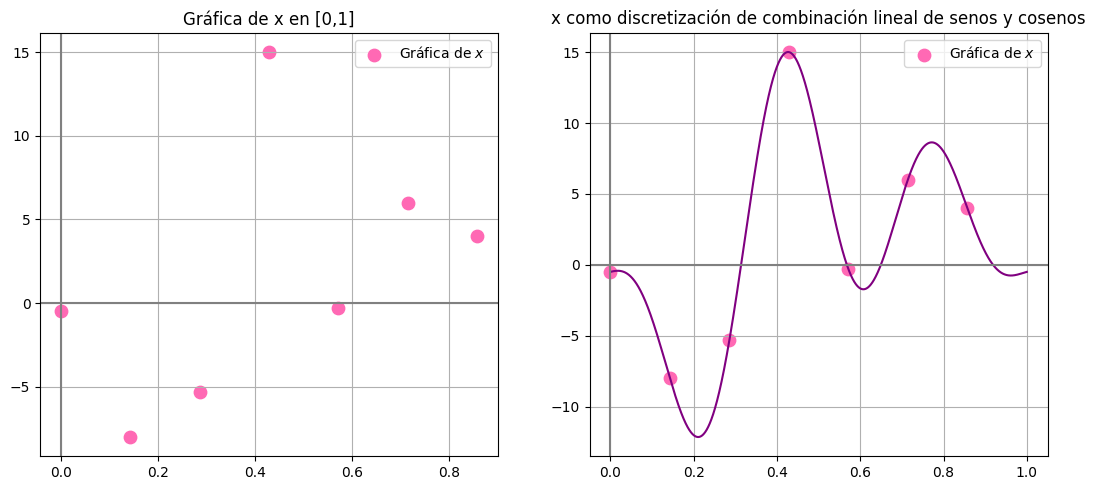
\includegraphics[scale=0.44]{ejFrecuencia_6} 
\end{figure}	
\final
\end{ejemplo}

Para terminar, digamos en concreto qué se entiende
por el espectro que resulta de usar la 
versión real de la transformada
discreta de fourier para analizar una señal finita.

En la definición 
$\cali{F}_{n}$ de la base dada en 
\ref{prop: base de fourier version real}, observe que, 
por cada frecuencia entera $\omega$ considerada,
aparecen uno o dos sinusoides (discretizados) con tal frecuencia:


\begin{table}[ht]
\sidecaption{Dimensión $n = 2M-1$ impar}
\centering
  \begin{tabular}{ l | c | c | c | c }
    \hline
    Frecuencia & $0$ & $1$ & $\ldots$ & $M-1$  \\ \hline
    Cant. sinusoides  & $1$ & $2$ & $\ldots$ & $2$ \\
    \hline
  \end{tabular}
\label{Tab: frecuencias TDF n impar}
\end{table}

\vspace{2cm}

\begin{table}[ht]
\sidecaption{Dimensión $n = 2M$ par}
\centering
  \begin{tabular}{ l | c | c | c | c | c}
    \hline
    Frecuencia & $0$ & $1$ & $\ldots$ & $M-1$ & $M$  \\ \hline
    Cant. sinusoides  & $1$ & $2$ & $\ldots$ & $2$ & $1$ \\
    \hline
  \end{tabular}
\label{Tab: frecuencias TDF n par}
\end{table}

\begin{defi}
\label{def. Dom tdf}
Sea $n \geq 2$. Llamaremos $Dom_{TDF, n}$ al conjunto de frecuencias
consideradas en la transformada discreta de Fourier para
las señales de dimensión $n$, o sea, al siguiente subconjunto de $\IR$;

\[
Dom_{TDF, n} = \{ 0 , 1, \cdots, M-1 \}
\hspace{0.2cm} \text{si } n = 2M-1
\hspace{0.2cm}
\text{es impar, }
\]
y
\[
Dom_{TDF, n} = \{ 0 , 1, \cdots, M \}
\hspace{0.2cm} \text{si } n = 2M-1
\hspace{0.2cm}
\text{es par.}
\]
\end{defi}


\begin{nota}
\label{nota: ya?}
Por ser 
la base de Fourier real
$\cali{F}_{n}$ una BON de $\IR^{n}$, 
si $M = \lceil \frac{n}{2} \rceil$,
\begin{equation}
\label{ec: sintesis 0}
x = \langle x , c_{n, 0} \rangle c_{n, 0} + \suma{\omega = 1}{M-1}{(
\langle x , c_{n, \omega} \rangle c_{n, \omega} + 
\langle x , s_{n, \omega} \rangle s_{n, \omega} )}
\hspace{0.2cm} \text{si n es impar}
\end{equation}

\begin{equation}
\label{ec: sintesis 1}
x = \langle x , c_{n, 0} \rangle c_{n, 0} + \suma{\omega = 1}{M-1}{(
\langle x , c_{n, \omega} \rangle  c_{n, \omega} + \langle x , s_{n, \omega} \rangle
s_{n, \omega} )}
+ \langle x , c_{n, M} \rangle c_{n, M} 
\hspace{0.2cm} \text{si n es par;}
\end{equation}

así, usando la transformada discreta de Fourier
-que, en este contexto, pensamos como calcular
los coeficientes de $x$ respecto a $\cali{F}_{n}$- 
tenemos tanto
un proceso de análisis de $x$ (que pensamos como
el cálculo de tales coeficientes)
respecto a sinusoides discretizados
de frecuencias $\omega \in Dom_{TDF, n}$
como uno de síntesis, que interpretamos como
el recuperar a la señal original $x$ usando
sus coeficientes respecto a $\cali{F}_{n}$.
\end{nota}

Se vale además la
identidad de Parseval, luego, para toda
señal $x \in \IR^{n}$,

\begin{equation}
\label{eq0: 25Ap}
||x||^{2} = \langle x , c_{n,0} \rangle^{2}+
\suma{\omega=0}{M-1}{(\langle x , c_{n,\omega} \rangle^{2} + 
\langle x , s_{n,\omega} \rangle^{2})}
\hspace{0.2cm} \textit{si n es impar} 
\end{equation}
y
\begin{equation}
\label{eq1: 25Ap}
||x||^{2} = \langle x , c_{n,0} \rangle^{2}+
\suma{\omega=0}{M-1}{(\langle x , c_{n,\omega} \rangle^{2} + 
\langle x , s_{n,\omega} \rangle^{2})}
+ \langle x , c_{n,M} \rangle^{2}
\hspace{0.2cm} \textit{si n es par};
\end{equation}
así, los coeficientes de la forma
$\langle x , c_{n,\omega} \rangle^{2}$ y 
$\langle x , s_{n,\omega} \rangle^{2}$
dan información sobre el peso que la frecuencia
$\omega$ tiene para sintetizar a la señal $x$.

\marginnote{Según las ecuaciones \eqref{eq0: 25Ap}
y \eqref{eq1: 25Ap}, los coeficientes $\tau_{n, \omega}(x)$
permiten calibrar la presencia de la frecuencia $\omega$
(en los rangos dados por las tablas 6.1 y 6.2)
en una señal $x$.}

\begin{defi}
\label{def: taus}
Sean $n \geq 2$, $M = \lceil \frac{n}{2} \rceil $.
Definimos
	\[
	\tau_{n}(x, 0) := \frac{|\langle x, c_{n,0} \rangle|}{|| x ||} ,	
	\]
	y
	\[
	\forall 
	\hspace{0.1cm}	
	1 \leq \omega \leq M-1: \hspace{0.2cm} 
	\tau_{n}(x, \omega) := 
	\frac{\sqrt{
	\langle x, c_{n,\omega} \rangle^{2}+
	\langle x, s_{n,\omega} \rangle^{2}}}{||x||}.	
	\]	
		Si $n$ es par, se define además a
	\[
	\tau_{n}(x, M) := 
	\frac{ |\langle x, c_{n,M} \rangle| }{ ||x|| }.
	\]
\end{defi}
De las ecuaciones 
\eqref{eq0: 25Ap} y 
\eqref{eq1: 25Ap} se deduce
fácilmente que, para toda $\omega$, 
$0 \leq \tau_{n}(x, \omega) \leq 1$. Puede pensar
a tales coeficientes $\tau_{n}(x, \omega)$ como la
contribución (normalizada por la norma de $x$)
de la frecuencia $\omega$ para sintetizar a $x$.


\begin{defi}
\label{def: espectro DFT}
Sean $n \geq 2$,  $x \in \IR^{n}$. Por el 
\textbf{espectro de $x$ 
obtenido a partir de la TDF} nos referiremos
a la 
función 
$\mathrm{T}_{x} : Dom_{TDF, n} \longrightarrow [0, 1] \subseteq \IR$
definida como
\[
\mathrm{T}_{x} (\omega) = \tau_{n}(x, \omega)
\hspace{0.2cm} \text{ para toda }
\hspace{0.2cm} \omega \in Dom_{TDF, n},
\]
donde los coeficientes $\tau_{n}(x, \omega)$
son como se definieron en \ref{def: taus}
\end{defi}

\begin{ejemplo}
A continuación se grafica el espectro
(a la derecha) obtenido
a partir de la TDF de la señal considerada en el 
ejemplo \ref{ej: DFT1}.

\begin{figure}[H]
	\sidecaption{
	Espectro de la señal $x$ dada en 
	\eqref{eq2: 10ab}. 
	\label{fig: dft_espectro_1}
	}
	\centering
	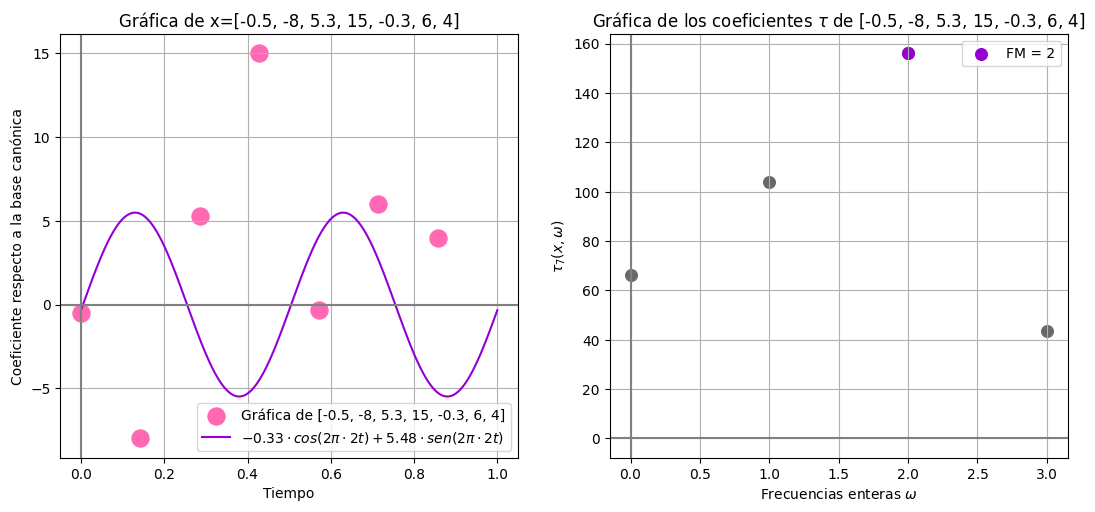
\includegraphics[scale = 0.45]{dft_espectro_1} 
\end{figure}	

Como se marca en el espectro con color morado, la frecuencia
asociada al coeficiente $\tau$ más alto es $\omega =2$; a la
izquierda, junto con la gráfica de la señal 
$x$, se dibuja el sinusoide (en versión continua)
de frecuencia $2$ que aparece en el análisis de
$x$ respecto a $\cali{F}_{7}$ dado en 
\eqref{eq: analisis x TDF}.
\final
\end{ejemplo}